\documentclass[review]{elsarticle}
%DIF LATEXDIFF DIFFERENCE FILE
%DIF DEL ../r1/paper.tex   Thu Jan 16 15:07:24 2020
%DIF ADD paper.tex         Mon Feb  3 09:29:54 2020

\usepackage{lineno,hyperref}
\modulolinenumbers[5]

\journal{Journal of Information Processing and Management}

%%%%%%%%%%%%%%%%%%%%%%%
%% Elsevier bibliography styles
%%%%%%%%%%%%%%%%%%%%%%%
%% To change the style, put a % in front of the second line of the current style and
%% remove the % from the second line of the style you would like to use.
%%%%%%%%%%%%%%%%%%%%%%%

%% Numbered
%\bibliographystyle{model1-num-names}

%% Numbered without titles
%\bibliographystyle{model1a-num-names}

%% Harvard
%\bibliographystyle{model2-names.bst}\biboptions{authoryear}

%% Vancouver numbered
%\usepackage{numcompress}\bibliographystyle{model3-num-names}

%% Vancouver name/year
%\usepackage{numcompress}\bibliographystyle{model4-names}\biboptions{authoryear}

%% APA style
%\bibliographystyle{model5-names}\biboptions{authoryear}

%% AMA style
%\usepackage{numcompress}\bibliographystyle{model6-num-names}

%% `Elsevier LaTeX' style
\bibliographystyle{elsarticle-num}
%%%%%%%%%%%%%%%%%%%%%%%

\usepackage{times}
\usepackage{latexsym}

\usepackage{url}

\usepackage{soul}
\usepackage{algorithm}
\usepackage{algorithmic}
\urlstyle{same}

\usepackage{helvet}
\usepackage{courier}
\usepackage{color}
\usepackage{amsmath,amsfonts,amssymb,amsthm,amsopn}
\usepackage{epsfig}
\usepackage{graphicx}
\usepackage{booktabs}
\usepackage{diagbox}
\usepackage{array}
\usepackage{multicol}
\usepackage{threeparttable}
\usepackage{epstopdf}
\usepackage{listings}
\usepackage{multirow}
\usepackage{subfigure}
\theoremstyle{definition}
\newtheorem{example}{Example}

\newcommand{\secref}[1]{Section \ref{#1}}
\newcommand{\figref}[1]{Figure \ref{#1}}
\newcommand{\eqnref}[1]{Eq. (\ref{#1})}
\newcommand{\tabref}[1]{Table \ref{#1}}
\newcommand{\exref}[1]{Example \ref{#1}}
\newcommand{\cut}[1]{}
\newcommand{\tabincell}[2]{\begin{tabular}{@{}#1@{}}#2\end{tabular}}

%\newcommand{\KZ}[1]{\textcolor{blue}{Kenny: #1}}
%\newcommand{\YZ}[1]{\textcolor{red}{Yizhu: #1}}
%DIF PREAMBLE EXTENSION ADDED BY LATEXDIFF
%DIF UNDERLINE PREAMBLE %DIF PREAMBLE
\RequirePackage[normalem]{ulem} %DIF PREAMBLE
\RequirePackage{color}\definecolor{RED}{rgb}{1,0,0}\definecolor{BLUE}{rgb}{0,0,1} %DIF PREAMBLE
\providecommand{\DIFaddtex}[1]{{\protect\color{blue}\uwave{#1}}} %DIF PREAMBLE
\providecommand{\DIFdeltex}[1]{{\protect\color{red}\sout{#1}}}                      %DIF PREAMBLE
%DIF SAFE PREAMBLE %DIF PREAMBLE
\providecommand{\DIFaddbegin}{} %DIF PREAMBLE
\providecommand{\DIFaddend}{} %DIF PREAMBLE
\providecommand{\DIFdelbegin}{} %DIF PREAMBLE
\providecommand{\DIFdelend}{} %DIF PREAMBLE
%DIF FLOATSAFE PREAMBLE %DIF PREAMBLE
\providecommand{\DIFaddFL}[1]{\DIFadd{#1}} %DIF PREAMBLE
\providecommand{\DIFdelFL}[1]{\DIFdel{#1}} %DIF PREAMBLE
\providecommand{\DIFaddbeginFL}{} %DIF PREAMBLE
\providecommand{\DIFaddendFL}{} %DIF PREAMBLE
\providecommand{\DIFdelbeginFL}{} %DIF PREAMBLE
\providecommand{\DIFdelendFL}{} %DIF PREAMBLE
%DIF HYPERREF PREAMBLE %DIF PREAMBLE
\providecommand{\DIFadd}[1]{\texorpdfstring{\DIFaddtex{#1}}{#1}} %DIF PREAMBLE
\providecommand{\DIFdel}[1]{\texorpdfstring{\DIFdeltex{#1}}{}} %DIF PREAMBLE
\newcommand{\DIFscaledelfig}{0.5}
%DIF HIGHLIGHTGRAPHICS PREAMBLE %DIF PREAMBLE
\RequirePackage{settobox} %DIF PREAMBLE
\RequirePackage{letltxmacro} %DIF PREAMBLE
\newsavebox{\DIFdelgraphicsbox} %DIF PREAMBLE
\newlength{\DIFdelgraphicswidth} %DIF PREAMBLE
\newlength{\DIFdelgraphicsheight} %DIF PREAMBLE
% store original definition of \includegraphics %DIF PREAMBLE
\LetLtxMacro{\DIFOincludegraphics}{\includegraphics} %DIF PREAMBLE
\newcommand{\DIFaddincludegraphics}[2][]{{\color{blue}\fbox{\DIFOincludegraphics[#1]{#2}}}} %DIF PREAMBLE
\newcommand{\DIFdelincludegraphics}[2][]{% %DIF PREAMBLE
\sbox{\DIFdelgraphicsbox}{\DIFOincludegraphics[#1]{#2}}% %DIF PREAMBLE
\settoboxwidth{\DIFdelgraphicswidth}{\DIFdelgraphicsbox} %DIF PREAMBLE
\settoboxtotalheight{\DIFdelgraphicsheight}{\DIFdelgraphicsbox} %DIF PREAMBLE
\scalebox{\DIFscaledelfig}{% %DIF PREAMBLE
\parbox[b]{\DIFdelgraphicswidth}{\usebox{\DIFdelgraphicsbox}\\[-\baselineskip] \rule{\DIFdelgraphicswidth}{0em}}\llap{\resizebox{\DIFdelgraphicswidth}{\DIFdelgraphicsheight}{% %DIF PREAMBLE
\setlength{\unitlength}{\DIFdelgraphicswidth}% %DIF PREAMBLE
\begin{picture}(1,1)% %DIF PREAMBLE
\thicklines\linethickness{2pt} %DIF PREAMBLE
{\color[rgb]{1,0,0}\put(0,0){\framebox(1,1){}}}% %DIF PREAMBLE
{\color[rgb]{1,0,0}\put(0,0){\line( 1,1){1}}}% %DIF PREAMBLE
{\color[rgb]{1,0,0}\put(0,1){\line(1,-1){1}}}% %DIF PREAMBLE
\end{picture}% %DIF PREAMBLE
}\hspace*{3pt}}} %DIF PREAMBLE
} %DIF PREAMBLE
\LetLtxMacro{\DIFOaddbegin}{\DIFaddbegin} %DIF PREAMBLE
\LetLtxMacro{\DIFOaddend}{\DIFaddend} %DIF PREAMBLE
\LetLtxMacro{\DIFOdelbegin}{\DIFdelbegin} %DIF PREAMBLE
\LetLtxMacro{\DIFOdelend}{\DIFdelend} %DIF PREAMBLE
\DeclareRobustCommand{\DIFaddbegin}{\DIFOaddbegin \let\includegraphics\DIFaddincludegraphics} %DIF PREAMBLE
\DeclareRobustCommand{\DIFaddend}{\DIFOaddend \let\includegraphics\DIFOincludegraphics} %DIF PREAMBLE
\DeclareRobustCommand{\DIFdelbegin}{\DIFOdelbegin \let\includegraphics\DIFdelincludegraphics} %DIF PREAMBLE
\DeclareRobustCommand{\DIFdelend}{\DIFOaddend \let\includegraphics\DIFOincludegraphics} %DIF PREAMBLE
\LetLtxMacro{\DIFOaddbeginFL}{\DIFaddbeginFL} %DIF PREAMBLE
\LetLtxMacro{\DIFOaddendFL}{\DIFaddendFL} %DIF PREAMBLE
\LetLtxMacro{\DIFOdelbeginFL}{\DIFdelbeginFL} %DIF PREAMBLE
\LetLtxMacro{\DIFOdelendFL}{\DIFdelendFL} %DIF PREAMBLE
\DeclareRobustCommand{\DIFaddbeginFL}{\DIFOaddbeginFL \let\includegraphics\DIFaddincludegraphics} %DIF PREAMBLE
\DeclareRobustCommand{\DIFaddendFL}{\DIFOaddendFL \let\includegraphics\DIFOincludegraphics} %DIF PREAMBLE
\DeclareRobustCommand{\DIFdelbeginFL}{\DIFOdelbeginFL \let\includegraphics\DIFdelincludegraphics} %DIF PREAMBLE
\DeclareRobustCommand{\DIFdelendFL}{\DIFOaddendFL \let\includegraphics\DIFOincludegraphics} %DIF PREAMBLE
%DIF LISTINGS PREAMBLE %DIF PREAMBLE
\lstdefinelanguage{codediff}{ %DIF PREAMBLE
  moredelim=**[is][\color{red}]{*!----}{----!*}, %DIF PREAMBLE
  moredelim=**[is][\color{blue}]{*!++++}{++++!*} %DIF PREAMBLE
} %DIF PREAMBLE
\lstdefinestyle{codediff}{ %DIF PREAMBLE
	belowcaptionskip=.25\baselineskip, %DIF PREAMBLE
	language=codediff, %DIF PREAMBLE
	basicstyle=\ttfamily, %DIF PREAMBLE
	columns=fullflexible, %DIF PREAMBLE
	keepspaces=true, %DIF PREAMBLE
} %DIF PREAMBLE
%DIF END PREAMBLE EXTENSION ADDED BY LATEXDIFF

\begin{document}

\begin{frontmatter}

\title{Reducing Repetition in Convolutional Abstractive Summarization}

%% Group authors per affiliation:
\author[mymainaddress]{Yizhu Liu}
\ead{liuyizhu@sjtu.edu.cn}
\author[mymainaddress]{Xinyue Chen} 
\ead{sherryicss@gmail.com}
\author[mysecondaryaddress]{Xusheng Luo} 
\ead{lxs140564@alibaba.com}
\author[mymainaddress]{Kenny Q. Zhu\corref{mycorrespondingauthor}}
\ead{kzhu@cs.sjtu.edu.cn}
\cortext[mycorrespondingauthor]{Corresponding author}
\address[mymainaddress]{Department of Computer Science and Engineering, Shanghai Jiao Tong University, Shanghai, China}
\address[mysecondaryaddress]{Search and Recommendation Team, Alibaba Group,
Hangzhou, China}

\begin{abstract}
%DIF < Convolutional sequence to sequence (CNN seq2seq) models
%DIF < have met great success in abstractive summarization. 
\DIFaddbegin \DIFadd{Convolutional sequence to sequence (CNN seq2seq) models
have met great success in abstractive summarization. 
}\DIFaddend %However, their outputs often contain repetitive word sequences and logical
%inconsistencies, limiting the practicality of their application.
%It is important for CNN seq2seq model to get the ability to 
%generate summaries without repetition in abstractive summarization. 
\DIFdelbegin \DIFdel{Repetition }\DIFdelend \DIFaddbegin \DIFadd{However, repetition }\DIFaddend is a persistent problem in the task of 
\DIFdelbegin \DIFdel{convolutional sequence to sequence (}\DIFdelend CNN seq2seq \DIFdelbegin \DIFdel{) }\DIFdelend abstractive summarization. 
In this paper, we identify the repetition problem in abstractive summarization and find the reasons behind \DIFaddbegin \DIFadd{the }\DIFaddend repetition problem.
%based on CNN seq2seq model and attention mechanism.
%The repetition is caused by decoders attending to the same locations in source document and attending to similar (but different) sentences in the source. 
We propose to reduce the repetition in summaries by 
Attention Filter mechanism (ATTF) and Sentence-level \DIFdelbegin \DIFdel{Backtraching }\DIFdelend \DIFaddbegin \DIFadd{Backtracking }\DIFaddend Decoder (SBD),
which dynamically redistributes attention over the input sequence as the output sentences are generated. 
The ATTF can record previously attended locations in the source document directly and prevent decoder from attending to these locations. The SBD prevents the decoder from generating similar sentences more than once via backtracking at test.
The proposed model outperforms the baselines 
%{\bf consistently} 
in terms of ROUGE score, repeatedness, \DIFaddbegin \DIFadd{correlation, }\DIFaddend and readability. 
The results show that this approach 
generates high-quality summaries with minimal repetition,
and makes the reading experience better.
\end{abstract}

\begin{keyword}
Abstractive summarization;
Repetition reduction;
\DIFdelbegin \DIFdel{Convolutionl }\DIFdelend \DIFaddbegin \DIFadd{Convolutional }\DIFaddend sequence-to-sequence model; Attention mechanism 
\end{keyword}

\end{frontmatter}
\linenumbers
\section{Introduction}
\label{sec:intro}

Abstractive summarization is the task of creating a short, accurate,
informative and fluent summary from a longer text document.
It attempts to reproduce the semantics and topics of original text
by paraphrasing. 
Recently, sequence to sequence
models~\cite{RushCW15,ChopraAR16,NallapatiZSGX16,SeeLM17,PaulusXS17}
have made great progress on abstractive summarization.
Recent study~\cite{bai2018empirical} suggests that, 
without additional, complicated structures or features,
convolutional sequence to sequence 
(CNN seq2seq) models~\cite{gehring2017convs2s,FanGA18,LiuLZ18} 
%DIF < CNN seq2seq models~\cite{gehring2017convs2s,FanGA18,LiuLZ18} 
%DIF < is a more powerful toolkit for sequence modeling than recurrent network.
are more effective and can be trained much faster due to 
its intrinsic parallel nature 
compared to recurrent \DIFdelbegin \DIFdel{networks (RNN )}\DIFdelend \DIFaddbegin \DIFadd{sequence-to-sequence seq2seq (RNN seq2seq) models}\DIFaddend .
Furthermore, unlike RNN-based models, 
the \DIFdelbegin \DIFdel{convolutional }\DIFdelend \DIFaddbegin \DIFadd{CNN-based }\DIFaddend models have more stable gradients 
because of \DIFdelbegin \DIFdel{its backpropagation paths}\DIFdelend \DIFaddbegin \DIFadd{their backpropagation paths~\mbox{%DIFAUXCMD
\cite{bai2018empirical, LiuLZ18}}\hspace{0pt}%DIFAUXCMD
}\DIFaddend . 
Thus, we take CNN seq2seq models as the target model to improve on and
compare with
in this paper.

Unfortunately, just like RNN-based models, CNN-based models also produce
summaries with substantial repeated word sequences which impacts the reading efficiency.
\tabref{tab:example} illustrates one 
test case from the CNN/Daily Mail summarization dataset. 
In this case, the basic CNN \DIFaddbegin \DIFadd{model }\DIFaddend produces two 
identical sentences (italized)\DIFdelbegin \DIFdel{in the result}\DIFdelend . 
Unlike machine translation or paraphrasing in which the output words
and input words are almost one-to-one aligned, the output of summarization
is ``compressed'' from the input document. Naturally, every sentence or 
word sequence in the summary corresponds to one or more places in the source
document. If there were two identical word sequences in the summary,
they might be looking at and summarizing the same ``spots'' in the source \DIFaddbegin \DIFadd{document}\DIFaddend .
This is evident from the attention map for the three sentences generated by 
\DIFdelbegin \DIFdel{CNN}\DIFdelend \DIFaddbegin \DIFadd{basic CNN model}\DIFaddend , shown in \figref{fig:attn_map}. 
The 1st and 3rd sentences attend to
the same location in the source (red boxes), while the second
sentence attends to another separate location in the source (green box). 
The two attention maps in the red boxes are very similar.

\begin{table}[th!]
\begin{center}
\scriptsize
\begin{tabular}{|l|}%{|p{7cm}|rl|}
\hline \bf Source document \\
\hline manchester city are rivalling manchester united and arsenal for valenciennes \\
       teenage defender dayot upamecano . the 16-year-old almost joined united in \\
	   the january transfer window only for him to opt to stay in france for a few \\
	   more months . centre-back umecano has played for france at u16 and u17 \\
	   level . monaco , inter milan and paris stgermain had also expressed interest. \\
	   fourth-placed city face aston villa at the etihad stadium on saturday . \\
\hline \bf Reference summary \\
\hline dayot upamecano was close to signing for manchester united in january . \\
       the 16-year-old, however , opted to stay in france with valenciennes . \\
	   centre-back upamecano has played for france at u16 and u17 level . \\
	   arsenal are also interested in the defender as man city join chase . \\
\hline \bf Basic CNN model (CNN) \\
\hline \textit{manchester city face aston villa at the etihad stadium on saturday .}\\
       the 16-year-old almost joined united in the january transfer window . \\
	   \textit{manchester city face aston villa at the etihad stadium on saturday .}\\
\hline
\end{tabular}
\end{center}
\caption{\label{tab:example} Summary generated by the basic CNN model}
\end{table}


\begin{figure}[th!]
\centering
\subfigure[Attention distribution]{
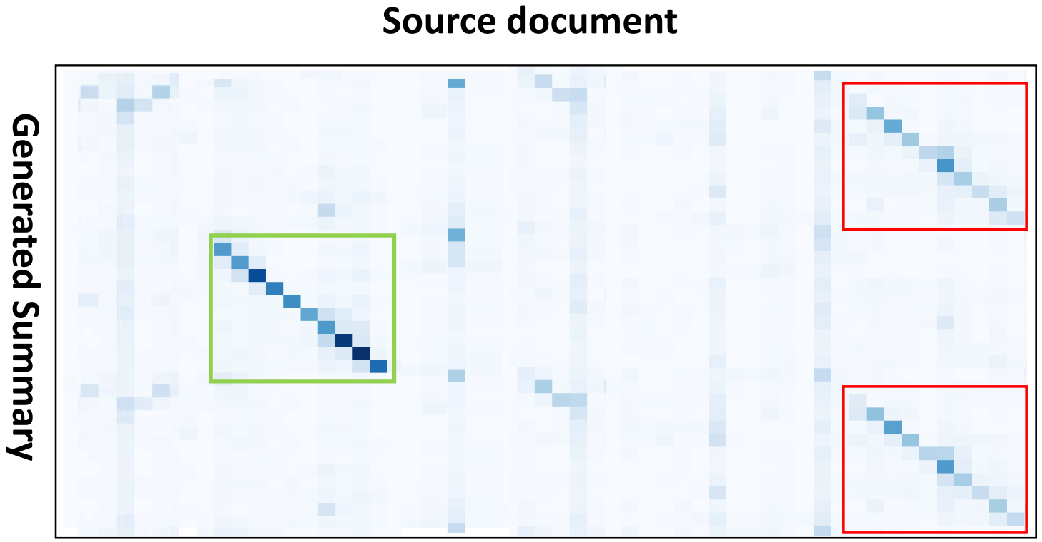
\includegraphics[width=0.8\linewidth]{map}
}
\quad
\subfigure[Green box]{
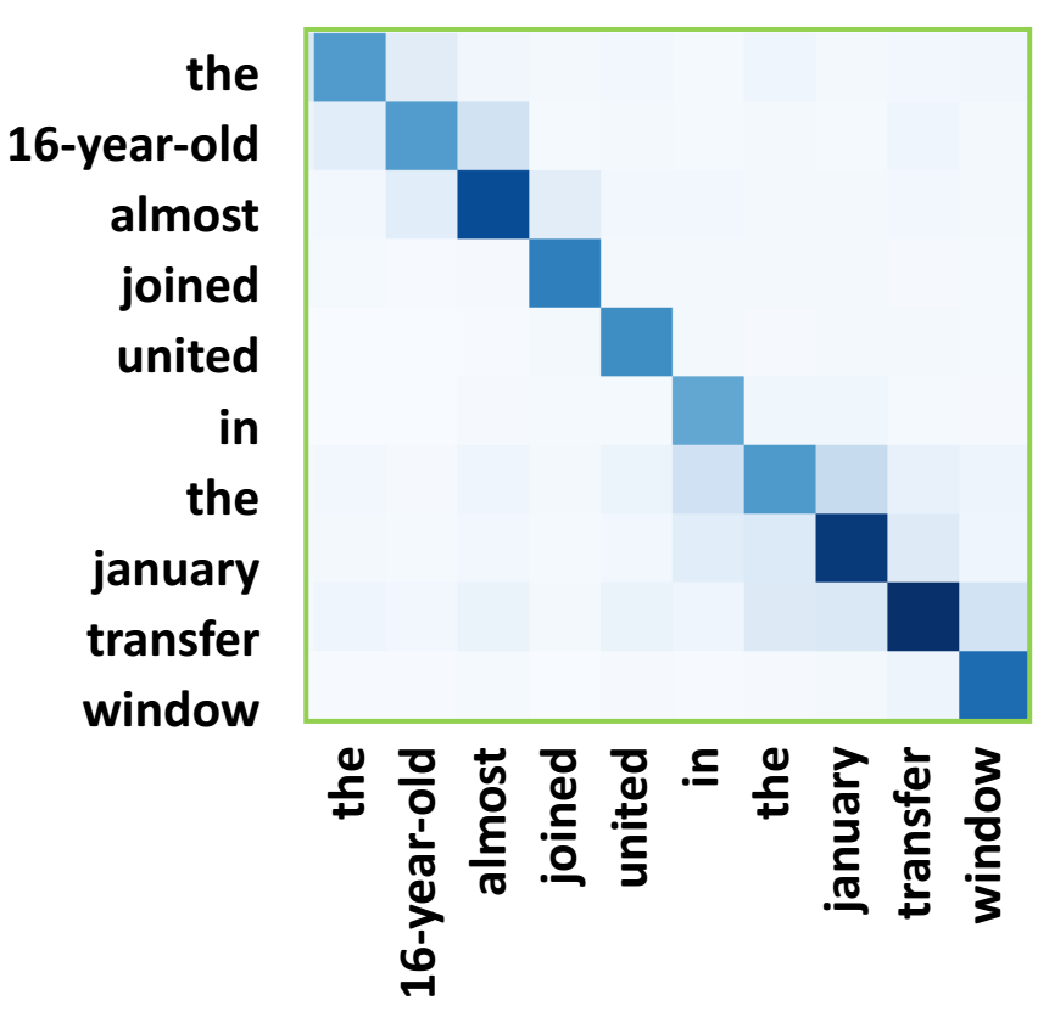
\includegraphics[width=0.44\linewidth]{map_1}
}
\quad
\subfigure[Red box]{
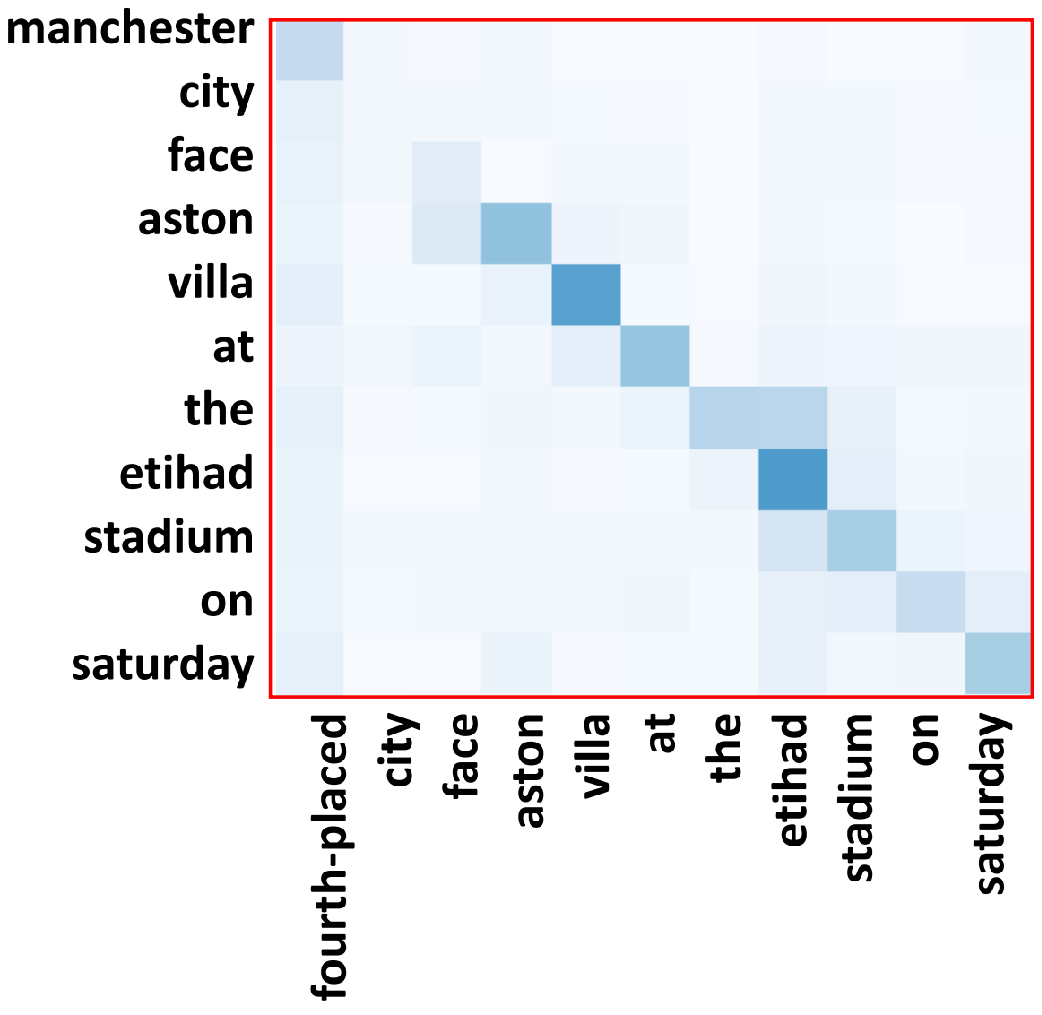
\includegraphics[width=0.44\linewidth]{map_2}
}
\caption{Attention for example on \DIFaddbeginFL \DIFaddFL{the basic }\DIFaddendFL CNN model in \tabref{tab:example}}
\label{fig:attn_map}
\end{figure}

Driven by this intuition, a few efforts have been made on ``remembering''
what has been focused on before at decoding. 
For example, 
Paulus~\cite{PaulusXS17} and 
Fan~\cite{FanGA18} use intra-temporal 
attention~\cite{NallapatiZSGX16} as well as intra-decoder attention to avoid
attending to the same parts in the source by 
revising attention scores while decoding. 
See~\cite{SeeLM17} and Gehrmann~\cite{GehrmannDR18}
respectively propose coverage mechanism and coverage penalty,
which records the sum of attention distributions of all previously generated words 
%DIF < to keep track of what has been summarized in different way.  
in a different way to track the summarized information.  
While these approaches discourage repetition to some extent,
they do so in an indirect manner. That is, they do not 
make use of the attention information in source directly.
Consequently, they may still generate repeated phrases, 
especially in long sentences (shown in the first 5 \DIFdelbegin \DIFdel{sections }\DIFdelend \DIFaddbegin \DIFadd{summaries }\DIFaddend of
\tabref{tab:strong_methods}).


\begin{table}[th!]
\begin{center}
\scriptsize
\begin{tabular}{|l|}%{|p{7cm}|rl|}

\hline \bf Intra-temporal attention (ITA) \\
\hline \textit{manchester city face aston villa at the etihad stadium on saturday .} \\
	   \textit{manchester city face aston villa at the etihad stadium on saturday .}\\
\hline \bf Intra-temporal $+$ Intra-decoder (ITDA) \\
\hline \textit{manchester city are rivalling manchester united and arsenal }for valenciennes\\
       teenage . manchester city face aston villa at the etihad stadium on saturday . \\
	   \textit{manchester city are rivalling manchester united and arsenal }. \\
\hline \bf Coverage model (COV) \\
\hline \textit{manchester city face aston villa at the etihad stadium on saturday .} \\
       manchester city are rivalling manchester united and arsenal for valenciennes . \\
	   \textit{manchester city face aston villa at the etihad stadium on saturday .}\\
\hline \bf Coverage penalty (COVP)\\
\hline \textit{manchester city face aston villa at the etihad stadium on saturday .}\\
       \textit{manchester city face aston villa at the etihad stadium on saturday .}\\
	   manchester city are rivalling manchester united and arsenal .\\
\hline \bf Semantic cohesion loss (SCL) \\
\hline \textit{manchester city are rivalling manchester united and arsenal for } defender dayot upamecano . \\
       \textit{manchester city are rivalling for} valenciennes teenage. \\
\hline \bf Trigram decoder (TRI) \\
\hline \underline{defender dayot upamecano} has played for \underline{france} at unk and unk level .\\ 
       manchester city face aston villa at the etihad stadium on saturday . \\
\hline \bf Ours (Attention Filter + Backtracking decoder) \\
\hline manchester city face aston villa at the etihad stadium on saturday . \\
       the 16-year-old almost joined united in the january transfer window . \\
	   manchester city are rivalling manchester united and arsenal for teenage defender daypot upamecano .\\
\hline
\end{tabular}
\end{center}
\caption{\label{tab:strong_methods} Generated summaries of the source in \tabref{tab:example}}
\end{table}

In this paper, we propose an attention filter mechanism that directly 
redistributes the attention from each word in the output summary to the source. 
It does so by computing the \DIFdelbegin \DIFdel{parts of interest }\DIFdelend \DIFaddbegin \textbf{\DIFadd{parts of interest}} \DIFaddend (POIs) in the source
per segment in the summary
\DIFdelbegin \DIFdel{~
%DIF < \footnote{In this paper, a segment means a sentence or clause delimited by punctuation.}, 
}\DIFdelend and then minimizing the attention scores of
words in these POIs that have already been attended to by the preceding 
segments during decoding. 
A segment means a sentence or clause delimited by punctuation,
which carries syntactic and semantic information. 
\DIFdelbegin \DIFdel{It }\DIFdelend \DIFaddbegin \DIFadd{This }\DIFaddend is very simple but effective \DIFaddbegin \DIFadd{way to split the summaries}\DIFaddend . 
Since punctuations 
play an important role in written language to organize 
the grammatical structures and to clarify the meaning of sentences~\cite{briscoe1996,Kim19,LiWE19}
%DIF < (Jones, 1996;Briscoe et al., 1997;Kim et al., 2019;Li et al., 2019).
Specifically, we calculate the attention in terms of segments, larger semantic units than tokens, 
which intuitively helps with emphasis of attention and POIs in source.
Different segments in summary thus do not attend to the same semantic spots
of source, and repetition is reduced. 
This is different from previous approaches
\DIFdelbegin \DIFdel{which }\DIFdelend \DIFaddbegin \DIFadd{that }\DIFaddend all do not exactly pinpoint these parts in the source,
which we believe is critical in reducing repetition. 
%DIF < This kind of partial attention 
%DIF < can help us to pinpoint the corresponding location that each segment is
%DIF < attending to. Then we use attention filter to filter
%DIF < a partial attention from normal attention of each tokens in the other sections
%DIF < by minimizing the attention scores of attended location in source document.
%DIF < This can optimize the alignment relationship between source document and 
%DIF < summarization.  This is shown in \tabref{tab:attn_exp}. 

Despite the above effort, there are cases, where similar sentences 
exist in the same source document:
\begin{example}
\label{ex:repeatsrc}
%DIF < \fbox{
%DIF < \parbox{0.9\columnwidth}{
\small{``..the standout fixture in the league on saturday sees leaders 
	   chelsea welcome manchester united ... chelsea midfielder oriol romeu, 
\textbf{currently on loan at stuttgart}, ... romeu is 
\textbf{currently on a season-long loan at bundesliga side stuttgart.}''} 
%DIF < }}
\end{example}

In this case, even if the decoder attends to different POIs of 
source document as it produces words, repetition may still result.  
At different timesteps,
the decoder may attend 
to sentences that are similar in different positions.
\DIFdelbegin \DIFdel{One }\DIFdelend \DIFaddbegin \DIFadd{There are two }\DIFaddend potential solution to this\DIFaddbegin \DIFadd{.
One }\DIFaddend is semantic cohesion loss~\cite{elikyilmazBHC18}
which takes the cosine similarity between two consecutively generated sentences
as part of the loss function. \DIFdelbegin \DIFdel{It }\DIFdelend \DIFaddbegin \DIFadd{However, it }\DIFaddend may attend to the same POI
and generate similar sentences (SCL row in \tabref{tab:strong_methods}).  
The other is a trigram decoder~\cite{PaulusXS17} 
which directly forbids repetition of previously generated trigrams at test time. 
While this simple but crude method avoids the repeat of any kind
completely, 
it ignores the fact that \textit{some amount of repetition} may exist
in natural summaries.  
On the other hand, the meddling of the beam search
\DIFaddbegin \DIFadd{~}\footnote{\DIFadd{Beam search is an iterative algorithm widely used to decode
summaries in neural-based abstractive summarization.
~\mbox{%DIFAUXCMD
\cite{beamsearch}}\hspace{0pt}%DIFAUXCMD
}}
\DIFaddend at run-time causes another problem: 
it tends to generate sentences that are logically incorrect. 
In \tabref{tab:strong_methods} (TRI row), the defender dayot didn't
really play for France, according to the source.
That is, the subject and object are mismatched.
So in this paper, we instead introduce a {\em sentence-level} backtracking decoder
that prohibits the repeat of the same sentence at test time.
\DIFaddbegin \DIFadd{Compared with trigram decoder, }{\em \DIFadd{sentence-level}} \DIFadd{backtracking decoder
does not impact
the process of beam search in the middle of a sentence, 
which can reduce factual errors and grammatical erros.
}\DIFaddend Our summary produced for the example is shown in last \DIFdelbegin \DIFdel{section }\DIFdelend \DIFaddbegin \DIFadd{summary }\DIFaddend of 
\tabref{tab:strong_methods}.

%DIF < In multiple-sentence summarization task, we observe that more often than not, repetition 
%DIF < occurs in the form of the same or similar sentences, rather than repetitive phrases 
%DIF < inside sentences. 
%DIF < On the other hand, it is prone to grammatical and factual errors(\tabref{tab:attn_exp}).
%DIF < Because it detects repetitive trigrams only by setting the 
%DIF < probability of the third word to zero. 
%DIF < It ignores that there are some same N-gram in the target summaries.
%DIF < The natural generation of a sentence is disturbed, giving rise to, 
%DIF < for example, mismatch of subject and object, and wrong phrases. 
%DIF < summarization is not a text generation problem which are are almost
%DIF < one-to-one correspondence between input and output words, it requires the model 
%DIF < has the ability to decide where to attend and where to ignore.
%DIF < The reason for repetition in abstractive summarization based on CNN seq2seq models is
%DIF < that the models always attend to the same location in the source document.
%DIF < As shown \tabref{tab:attn_exp} 
%DIF < and \figref{fig:attn_map} are corresponding. 
%DIF < Sentence in blue has factual erro. and \figref{fig:attn_map}.
%DIF < In the attention map, the darker color, the higher attention score.
%DIF < the repeated sentence in summary attends to the same location
%DIF < with high attention score, and different sentences attend to different location in source document. 
%DIF < 
\DIFdelbegin %DIFDELCMD < 

%DIFDELCMD < %%%
%DIF < Zhou~\cite{ZhouYWZ17} pointed out that there is no obvious alignment relationship 
%DIF < between the source text and the target summary, 
%DIF < and the encoder outputs contain noise for the attention. 
%DIF < Thus, removing repetition in abstractive summarization on CNN seq2seq model
%DIF < need a strong attention mechamism that can get alignment relationship
%DIF < between source document and target summary and determine the summarized
%DIF < parts in source documents directly. 
%DIFDELCMD < 

%DIFDELCMD < \cut{%%%%%%%%%%%%%%%%
%DIFDELCMD < as shown in \tabref{tab:src_rep}.
%DIFDELCMD < \figref{fig:attn_map3} shows that the repeated sentences
%DIFDELCMD < in summary respectively attend to the similar sentences in source document.
%DIFDELCMD < So we force our decoder to never output the same sentence more than once by a sentence level
%DIFDELCMD < backtraching decoder during testing. 
%DIFDELCMD < 

%DIFDELCMD < \begin{table}[th!]
%DIFDELCMD < \begin{center}
%DIFDELCMD < \small
%DIFDELCMD < \begin{tabular}{lclclclc}%{|p{7cm}|rl|}
%DIFDELCMD < \hline \bf Source document \\
%DIFDELCMD < \hline chelsea 's on loan midfielder oriol romeu goes up against sportsmail 's \\
%DIFDELCMD <        martin ... . the standout fixture in the league on saturday sees leaders \\
%DIFDELCMD < 	   chelsea welcome manchester united to stamford bridge , ... \\
%DIFDELCMD < 	   chelsea midfielder oriol romeu , \textbf{currently on loan at stuttgart} , predicts \\
%DIFDELCMD < 	   the scores for the weekend 's matches . romeu is \textbf{currently on a season-long} \\
%DIFDELCMD < 	   \textbf{loan at bundesliga side stuttgart .} \\
%DIFDELCMD < \hline \bf Reference summary \\
%DIFDELCMD < \hline oriol romeu is on a season-long loan at stuttgart from chelsea . the spanish \\
%DIFDELCMD <        midfielder predicts the scores in saturday 's matches . romeu goes \\
%DIFDELCMD < 	   head-to-head with sportsmail 's martin keown . \\
%DIFDELCMD < \hline \bf Our (Attention Filter)\\
%DIFDELCMD < \hline chelsea beat manchester united on saturday . oriol romeu is currently \\
%DIFDELCMD <        on a season-long loan at stuttgart . oriol romeu is \\
%DIFDELCMD < 	   currently on a season-long loan at the end of the season .\\
%DIFDELCMD < \hline \bf Our (Attention Filter + Backtracking decoder) \\
%DIFDELCMD < \hline chelsea face manchester united in the premier league on saturday . oriol romeu \\
%DIFDELCMD <        is currently on loan at stuttgart . \\
%DIFDELCMD < \hline
%DIFDELCMD < \end{tabular}
%DIFDELCMD < \end{center}
%DIFDELCMD < \caption{\label{tab:src_rep} Summaries generated by source document with repeatedness. }
%DIFDELCMD < \end{table}
%DIFDELCMD < 

%DIFDELCMD < \begin{figure}[th!]
%DIFDELCMD < \centering
%DIFDELCMD < 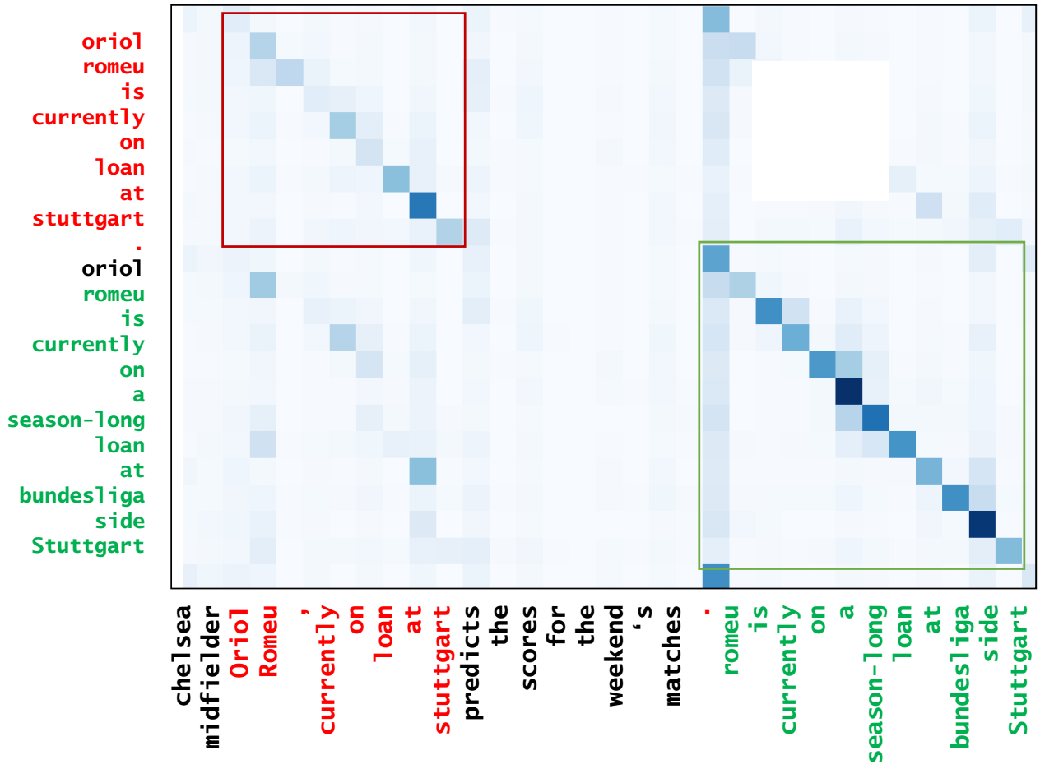
\includegraphics[width=0.9\linewidth]{map3}
%DIFDELCMD < \caption{Attention distribution(local) for our attention filter model in \tabref{tab:src_rep}}
%DIFDELCMD < \label{fig:attn_map3}
%DIFDELCMD < \end{figure}
%DIFDELCMD < }%%%
%DIF < %%%%%%%%%%%%%%%%%
%DIF < Compared with trigram decoder, we do not impact
%DIF < the process of beam search in the middle of a sentence, 
%DIF < which can reduce factual errors and grammatical erros(\tabref{tab:attn_exp}).
%DIFDELCMD < 

%DIFDELCMD < %%%
\DIFdelend Reducing repetition in abstractive summarization provides high-quality summaries for users and improves their reading efficiency.
We expect that other natural language generation (NLG) tasks with repetition problem can be \DIFdelbegin \DIFdel{enhances with our }\DIFdelend \DIFaddbegin \DIFadd{enhanced with our proposed }\DIFaddend approach. 
Our contributions are summarized as follows:
\begin{enumerate}
\item We identify the repetition problem in abstractive summaries generated
by CNN seq2seq models and find the reasons behind the repetition problem.
\item We propose new metrics to evaluate this problem: Repeatedness and Readability.
\item We propose an effective approach that redistributes attention scores 
during training time, and prevents repetition by sentence backtracking
at \DIFdelbegin \DIFdel{runtime }\DIFdelend \DIFaddbegin \DIFadd{test time }\DIFaddend to reduce repetition in CNN seq2seq model.
\item Our approach
outperforms the state-of-the-art (SOTA) CNN-based baselines 
substantially by all evaluation metrics, including ROUGE scores, 
repeatedness\DIFaddbegin \DIFadd{, correlation }\DIFaddend and readability.
\end{enumerate}

%DIF < Next, we present our approach based on convolutional sequence to sequence 
%DIF < model, followed by the evaluation of our approach and a discussion
%DIF < of related work. 
 \DIFaddbegin \DIFadd{Next, we discuss the related work (}\secref{sec:related}\DIFadd{),
followed by 
our approach based on convolutional sequence to sequence 
model (}\secref{sec:approach}\DIFadd{)
and the evaluation of our approach (}\secref{sec:eval}\DIFadd{).
 }\DIFaddend
\section{Related Work}
\label{sec:related}

%DIF < Summarization is the task of condensing a piece of document into a shorter paragraph or a single sentence, while retaining correctness, fluency, consistency as well as the core idea of the original document. 
\DIFdelbegin %DIFDELCMD < 

%DIFDELCMD < %%%
%DIF < Generally, this task is tackled in two different ways: extractive and abstractive. Extractive approach \cite{Dorr2003HedgeTA,DBLP:journals/corr/NallapatiZZ16} takes sentences from the source text to compose a summary, while abstractive one \cite{RushCW15,SeeLM17,PaulusXS17} \textit{generates} sentences word by word after comprehending the source text as a whole. For abstractive method, the algorithm has a vocabulary from which it can freely choose words and phrases to compose sentences, while the extractive one is more similar to catching the key sentences of the source text. Extractive summarization can more easily produce acceptable summaries, as copying sentences from the source text guarantees correctness and consistency. However, extractive methods lacks creativity. More often than not, humans summarize documents in an abstractive manner, where they comprehend the whole document before selecting elements from their vocabulary to compose a short text that encapsulates the main idea and even the underlying intent from the source sentences. This is where a sense of expressiveness and elegance can be found.
%DIFDELCMD < 

%DIFDELCMD < %%%
%DIF < Many \cite{RushCW15,SeeLM17} choose to build an abstractive model using sequence-to-sequence model using recurrent neural networks and attention mechanism. In pursuit of speed and  parallelism, \cite{gehring2017convs2s} proposed a convolutional seqence-to-sequence model with Gated Linear Units \cite{DauphinFAG17}, attention mechanism to tackle a series of generation tasks. It achieves state-of-the-art accuracy in abstractive single-sentence summarization and is much faster than recurrent approaches.
%DIFDELCMD < 

%DIFDELCMD < %%%
%DIF < Repetition is a persistent problem in the task of summarization. Models are found to in some cases generate similar or the same words and phrases repeatedly, which causes grammatical incorrectness and redundancy. This reflects a insufficiency in the decoder's awareness of previous generations. To address this issue,  \cite{SeeLM17} use coverage to keep track of what has been summarized, which discourages repetition in an indirect manner, \cite{PaulusXS17} propose intra-decoder attention to avoid attending to the same parts in the source text by dynamically revising attention scores while decoding. \cite{PaulusXS17} also avoid repetition in test time by directly banning the generation of repeated trigrams in beam search. However, the weakness of this method is that the action of eliminating highly probable sentences with repeated trigrams disturbs the process of beam search, giving rise to grammatically incorrect sentences, whose probabilities are actually low in the model. 
%DIFDELCMD < 

%DIFDELCMD < %%%
\DIFdel{Repetition problems 
is tackled in broadly two aspects }\DIFdelend \DIFaddbegin \DIFadd{Abstractive Summarization
is one of the most challenging and interesting problems 
in the field of Natural Language Processing (NLP)
\mbox{%DIFAUXCMD
\cite{CareniniC08,PallottaDB09,SankarasubramaniamRG14,BingLLLGP15,RushCW15,LiHZ16,YaoWX17,MohamedO19,LierdeC19,NguyenCNN19}}\hspace{0pt}%DIFAUXCMD
.
It is a process of generating a concise and meaningful summary of text from multiple text resources 
such as news articals.
Great progress~
\mbox{%DIFAUXCMD
\cite{RushCW15,ChopraAR16,NallapatiZSGX16,SeeLM17,PaulusXS17,HardyV18,KourisAS19,LiuL19,ZhangWZ19,WangQW19}
}\hspace{0pt}%DIFAUXCMD
has been made recently on
neural-based abstractive summarization.
Repetition is a persistent problem in the task of 
neural-based summarization. 
It is tackled broadly in two directions }\DIFaddend in recent years. 

\DIFdelbegin \DIFdel{Chen and Bansal}%DIFDELCMD < \shortcite{P18-1063} %%%
\DIFdel{and Li}%DIFDELCMD < \shortcite{D18-1205,D18-1441} %%%
\DIFdel{construct hierarchical models to deal with summarization. Their approaches typically involve information selection}\DIFdelend \DIFaddbegin \DIFadd{One involves }{\em \DIFadd{information selection}} \DIFaddend or sentence
selection before generating summaries.
\DIFdelbegin \DIFdel{Among them, }\DIFdelend \DIFaddbegin \DIFadd{Chen~}\DIFaddend \cite{P18-1063} uses an extractor  
\DIFdelbegin \DIFdel{agent }\DIFdelend to select salient sentences or highlights \DIFdelbegin \DIFdel{, }\DIFdelend and then employs 
an abstractor network to \DIFdelbegin \DIFdel{compress }\DIFdelend \DIFaddbegin \DIFadd{rewrite }\DIFaddend these sentences.
\DIFdelbegin \DIFdel{In their model, repetition is naturally avoided as long as the source document is non-repetitive. But it does not aim to }\DIFdelend \DIFaddbegin \DIFadd{It can not }\DIFaddend solve repetition in \DIFdelbegin \DIFdel{sequence-to-sequence generation (source document to summary).
\mbox{%DIFAUXCMD
\cite{D18-1205,D18-1441} }\hspace{0pt}%DIFAUXCMD
generate sentence representations and then use them to produce sentences for summary. All of the above models are RNN-based. 
However, 
their methods cannot be transferred easily to CNN-based models because there is no natural CNN-based approach to generate a sentence from a sentence }\DIFdelend \DIFaddbegin \DIFadd{seq2seq model.
Tan~\mbox{%DIFAUXCMD
\cite{TanWX17} }\hspace{0pt}%DIFAUXCMD
and Li~\mbox{%DIFAUXCMD
\cite{D18-1205,D18-1441} }\hspace{0pt}%DIFAUXCMD
encode
sentence using word vectors
and predicts words from sentence vector in sequential order 
whereas CNN-based models are naturally parallelized. 
While transferring RNN-based model to CNN model, 
the kernel size and the number of 
convolutional layers can not be easily determined when
converting between sentence and word }\DIFaddend vector. 
Therefore, we do not \DIFdelbegin \DIFdel{consider the above models as our baselines}\DIFdelend \DIFaddbegin \DIFadd{compare our models to those models}\DIFaddend . 

\DIFdelbegin \DIFdel{See}%DIFDELCMD < \shortcite{SeeLM17}%%%
\DIFdel{, Paulus}%DIFDELCMD < \shortcite{PaulusXS17} %%%
\DIFdel{and Fan}%DIFDELCMD < \shortcite{FanGA18} %%%
\DIFdel{choose to adopt sequence-to-sequence approach, where source document and
summary are treated as two long sequences, without the idea of separate sentences.
\mbox{%DIFAUXCMD
\cite{SeeLM17} }\hspace{0pt}%DIFAUXCMD
integrate coverage }\DIFdelend \DIFaddbegin \DIFadd{The other direction is to improve the 
}{\em \DIFadd{memory of previously generated words}}\DIFadd{.
Suzuki~\mbox{%DIFAUXCMD
\cite{SuzukiN17} }\hspace{0pt}%DIFAUXCMD
and Lin~\mbox{%DIFAUXCMD
\cite{LinSMS18} 
}\hspace{0pt}%DIFAUXCMD
deal with word repetition in single-sentence summaries, 
while we primarily deal with multi-sentence summaries with 
sentence-level repetition. 
%DIF > There is almost no word repetition in CNN-based model.
There is almost no word repetition in multi-sentence summaries.
Jiang~\mbox{%DIFAUXCMD
\cite{JiangB18} }\hspace{0pt}%DIFAUXCMD
adds a new decoder without attention mechanism.
In CNN-based model, attention mechanism is necessary to connect encoder 
and decoder.
Thus, our model also is not compared with the above models. 
The following models can be transferred to CNN seq2seq model and
are used as our baselines.
See~\mbox{%DIFAUXCMD
\cite{SeeLM17} }\hspace{0pt}%DIFAUXCMD
integrates coverage mechanism}\DIFaddend , 
which keeps track of what \DIFdelbegin \DIFdel{has }\DIFdelend \DIFaddbegin \DIFadd{have }\DIFaddend been summarized, as a feature that helps 
redistribute the attention \DIFdelbegin \DIFdel{score }\DIFdelend \DIFaddbegin \DIFadd{scores }\DIFaddend in an indirect manner\DIFaddbegin \DIFadd{,
}\DIFaddend in order to discourage repetition. 
\DIFdelbegin \DIFdel{\mbox{%DIFAUXCMD
\cite{PaulusXS17} }\hspace{0pt}%DIFAUXCMD
propose }\DIFdelend \DIFaddbegin \DIFadd{Tan~\mbox{%DIFAUXCMD
\cite{TanWX17} }\hspace{0pt}%DIFAUXCMD
uses distraction attention
\mbox{%DIFAUXCMD
\cite{ChenZLWJ16}}\hspace{0pt}%DIFAUXCMD
, which is identical to coverage mechanism. 
Gehrmann~\mbox{%DIFAUXCMD
\cite{GehrmannDR18} }\hspace{0pt}%DIFAUXCMD
adds coverage penalty to loss function
which increases whenever the decoder directs more than 1.0 of total attention
towards a word in encoder.
This penalty indirectly revises attention distribution and results in
the reduction of repetition.
}{\DIFadd{\c{C}}}\DIFadd{elikyilmaz~\mbox{%DIFAUXCMD
\cite{elikyilmazBHC18} }\hspace{0pt}%DIFAUXCMD
uses semantic cohesion loss,
which is the cosine similarity between two consecutive sentences, as part of
the loss that helps reduce repetition.
Paulus~\mbox{%DIFAUXCMD
\cite{PaulusXS17} }\hspace{0pt}%DIFAUXCMD
proposes }\DIFaddend intra-temporal attention \DIFaddbegin \DIFadd{\mbox{%DIFAUXCMD
\cite{NallapatiZSGX16} }\hspace{0pt}%DIFAUXCMD
}\DIFaddend and 
intra-decoder attention \DIFdelbegin \DIFdel{that dynamically revises }\DIFdelend \DIFaddbegin \DIFadd{which dynamically revises the }\DIFaddend attention distribution while decoding. 
\DIFdelbegin \DIFdel{\mbox{%DIFAUXCMD
\cite{PaulusXS17} }\hspace{0pt}%DIFAUXCMD
also avoid repetition in }\DIFdelend \DIFaddbegin \DIFadd{It also avoids repetition at }\DIFaddend test time by directly banning the generation of 
repeated trigrams in beam search. 
\DIFdelbegin \DIFdel{These two models are RNN-based. }\DIFdelend %DIF > These two models are RNN-based. 
\DIFaddbegin \DIFadd{Fan~}\DIFaddend \cite{FanGA18} borrows the idea from \DIFdelbegin \DIFdel{\mbox{%DIFAUXCMD
\cite{PaulusXS17} }\hspace{0pt}%DIFAUXCMD
and build a RNN-based model. 
We transfer methods from these models to form our baselines, as introduced in }%DIFDELCMD < \secref{sec:basic}%%%
\DIFdel{.
}\DIFdelend \DIFaddbegin \DIFadd{Paulus~\mbox{%DIFAUXCMD
\cite{PaulusXS17} }\hspace{0pt}%DIFAUXCMD
and 
builds a CNN-based model. 
}\DIFaddend 

Our model \DIFdelbegin \DIFdel{also adopts a sequence-to-sequence approach and }\DIFdelend deals with the attention in \DIFaddbegin \DIFadd{both }\DIFaddend encoders and decoders. 
Different from the previous methods, 
our \textit{attention filter mechanism} does not 
\DIFdelbegin \DIFdel{deal with }\DIFdelend \DIFaddbegin \DIFadd{treat }\DIFaddend the attention history \DIFdelbegin \DIFdel{collectively. Instead,  
our attention filter is section-aware. 
In \mbox{%DIFAUXCMD
\cite{SeeLM17,gehring2017convs2s}}\hspace{0pt}%DIFAUXCMD
}\DIFdelend \DIFaddbegin \DIFadd{as a whole data structure,  
but divides it into sections (}\figref{fig:model_main}\DIFadd{). 
%DIF > \KZ{I actually think it might be better to draw a diagram
%DIF > to show this in approach.} 
Previously}\DIFaddend , the distribution curve of accumulated attention scores 
for each token in the source document \DIFdelbegin \DIFdel{grows flatwith critical information washed away }\DIFdelend \DIFaddbegin \DIFadd{tends to be flat, 
which means critical information is washed out }\DIFaddend during decoding.
Our method \DIFdelbegin \DIFdel{, on the other hand, amplifies most }\DIFdelend \DIFaddbegin \DIFadd{emphasizes }\DIFaddend previously attended sections 
so that \DIFaddbegin \DIFadd{important }\DIFaddend information is retained\DIFdelbegin \DIFdel{(}%DIFDELCMD < \secref{sec:attf}%%%
\DIFdel{).
Also, given }\DIFdelend \DIFaddbegin \DIFadd{.
}

\DIFadd{Given }\DIFaddend our observation that repetitive sentences in the source \DIFdelbegin \DIFdel{is }\DIFdelend \DIFaddbegin \DIFadd{are
}\DIFaddend another cause for repetition in summary, 
which cannot be directly resolved by manipulating attention \DIFaddbegin \DIFadd{values}\DIFaddend , 
we introduce \DIFdelbegin \DIFdel{our }\DIFdelend \textit{sentence-level backtracking decoder}. 
Unlike \DIFaddbegin \DIFadd{Paulus }\DIFaddend \cite{PaulusXS17}, 
we do not ban repetitive \textit{trigrams} in test time. 
\DIFdelbegin \DIFdel{Instead, our }\DIFdelend %DIF > Instead, 
\DIFaddbegin \DIFadd{Our }\DIFaddend decoder regenerates a sentence that is similar to \DIFdelbegin \DIFdel{any }\DIFdelend previously generated ones.
With the two \DIFdelbegin \DIFdel{methods}\DIFdelend \DIFaddbegin \DIFadd{modules}\DIFaddend , our model is capable of generating summaries with \DIFaddbegin \DIFadd{a
}\DIFaddend natural level of repetition while retaining fluency and consistency.
 %DIF < plz let me know if revised or reused
\DIFdelbegin %DIFDELCMD < 

%DIFDELCMD <  %%%
\DIFdelend
\section{Approach}
\label{sec:approach}

In this section, we describe the model architecture used for our experiments
%and propose our reducing repetition method which is implemented by extending thebasic model.
and propose our novel repetition reduction method, which is an extension to the basic model.
~\footnote{
All of the data and source code
can be downloaded from http://202.120.38.146/sumrep.}

In summarization task, the input (source document) and
output (summary) are both sequences of words.
%DIF < \XS{elements? better use words or terms}.
Suppose the input and output are respectively represented as
$\textbf{x} = (x_{1},x_{2},...,x_{m})$ and 
$\textbf{y} = (y_{1}, y_{2},..., y_{n})$ ($m>n$),
the goal is to maximize the conditional probability
$p(\textbf{y}|\textbf{x})$:
\begin{equation}
\small
p(\textbf{y} | \textbf{x}) \!=\! {\prod\DIFdelbegin \DIFdel{^T}\DIFdelend \DIFaddbegin \DIFadd{^n}\DIFaddend _{t} {p(y_{t} | y_{1}, y_{2},..., y_{t-1}, \textbf{x}})}
\end{equation}

%Our goal is to model the above conditional probability in such a way that the 
Furthermore, we aim to generate summaries that are not only fluent 
and logically consistent with source document, but also with 
a small amount of repeatedness, which is natural in human written summaries.  
%(results illustrated in \tabref{tab:eval_repe}). 
%We aim at getting the above conditional probability which can generate summaries without repetition.

\subsection{Basic CNN seq2seq Model}
\label{sec:basic}
Our basic model is multi-layer convolutional seq2seq networks \cite{gehring2017convs2s} with attention mechanism.
\footnote{\url{https://github.com/facebookresearch/fairseq-py}}, 
as illustrated in \figref{fig:basicModel}. 

\begin{figure}[th]
    \centering
    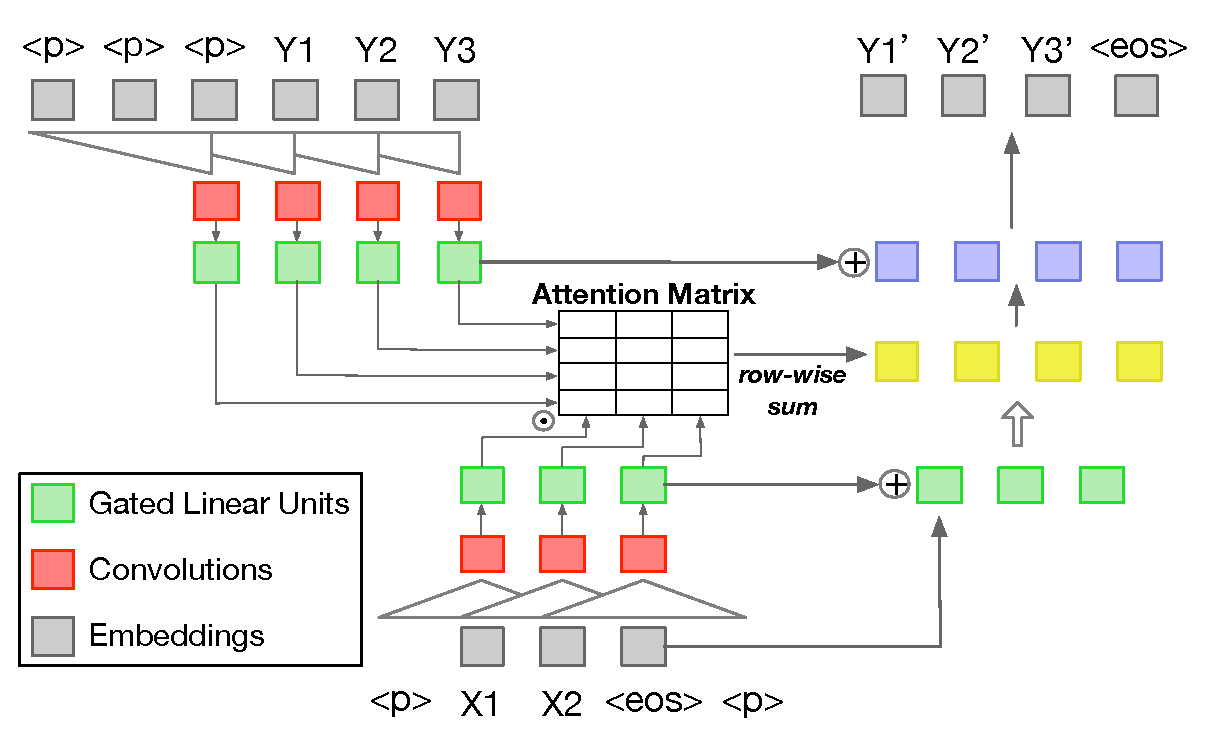
\includegraphics[width=0.8\linewidth]{cnn}
    \caption{Convolutional seq2seq model.}
	%$\odot$ stands for inner product. $\oplus$ stands for element-wise addition.}
    \label{fig:basicModel}
\end{figure}

%Our basic model includes multi-layer convolutional seq2seq networks \cite{gehring2017convs2s} and attention mechanism \footnote{\url{https://github.com/facebookresearch/fairseq-py}}, as illustrated in \figref{fig:basicModel}. 

For CNN seq2seq models, we combine both word embeddings and position embeddings to obtain input $\mathbf{X} = (X_1,...,X_m)$ and output $\mathbf{Y}=(Y_1,...,Y_n)$. 
%We denote $\mathbf { z } ^ { l }$ and $\mathbf { h } ^ { l }$ 
We denote $\mathbf { z } ^ { l } = \left( z _ { 1 } ^ { l } , \ldots , z _ { m     } ^ { l } \right)$ and $\mathbf { h } ^ { l } = \left( h _ { 1 } ^ { l } , \ldots , h _ { n } ^ { l } \right)$ 
respectively as convolutional output of the encoder and
decoder in the $l$-th layer.
%where $\mathbf { z } ^ { l } = \left( z _ { 1 } ^ { l } , \ldots , z _ { m } ^ { l } \right)$ and $\mathbf { h } ^ { l } = \left( h _ { 1 } ^ { l } , \ldots , h _ { n } ^ { l } \right)$. 
Each element of the output
sequence generated by the decoder network is fed
back into the next layer of decoder network.
In each layer, GLU \cite{DauphinFAG17} and residual connections \cite{HeZRS16}
are used respectively as a non-linear gate and guarantee for sufficient depth of the network.  
\begin{equation}
\small
    h _ { i } ^ { l } = GLU \left( W ^ { l } \left[ h _ {i-k/2 } ^ { l - 1 } , \ldots , h _ { i+k/2 } ^ { l - 1 } \right] + b _ { w } ^ { l } \right) + h _ { i } ^ { l - 1 }
\end{equation} 
where \textit{k} is kernel width. \DIFaddbegin \DIFadd{$W$ and $b$ are trainable parameters.
}\DIFaddend Next, we compute the probability distribution for the next word
using the top decoder output:
\begin{equation}
\small
    p \left( y _ { i + 1 } | y _ { 1 } , \ldots , y _ { i } , \mathbf { x } \right) = \operatorname { softmax } \left( W _ { o } h _ { i } ^ { L } + b _ { o } \right)
\end{equation}

For each decoder layer, the multi-step attention integrates encoder information. 
We compute decoder state $d_{i}^{l}$ for attention via
\begin{equation}
\small
    d _ { i } ^ { l } = W _ { d } ^ { l } h _ { i } ^ { l } + b _ { d } ^ { l } + Y _ { i }
\end{equation}

\begin{equation}\label{eq:a}
\small
    a _ { i j } ^ { l } = \frac { \exp \left( d _ { i } ^ { l } \cdot z _ { j } ^ { u } \right) } { \sum _ { t = 1 } ^ { m } \exp \left( d _ { i } ^ { l } \cdot z _ { t } ^ { u } \right) }
\end{equation}
\begin{equation}\label{eq:c}
\small
    c _ { i } ^ { l } = \sum _ { j = 1 } ^ { m } a _ { i j } ^ { l } \left( z _ { j } ^ { u } + X_j \right)
\end{equation}
%where $z_{j}^{u}$ is the encoder output of last layer $u$.  
where $d_{i}^{l}$ is decoder state, $z_{j}^{u}$ is the encoder state, 
$u$ is the last layer of encoder
and $a_{ij}$ is attention score.
The inner product between decoder state and encoder outputs is used 
to measure the affinity. 
The conditional input to the current 
decoder layer is a weighted sum of encoder states and input representations.
Finally, $c _ { i } ^ { l }$ is added to $h_{i}^{l}$, which forms the input for the next decoder layer or the final output.

\subsection{Attention Filter Mechanism (ATTF)}
\label{sec:attf}

\begin{figure}[th]
	\centering
	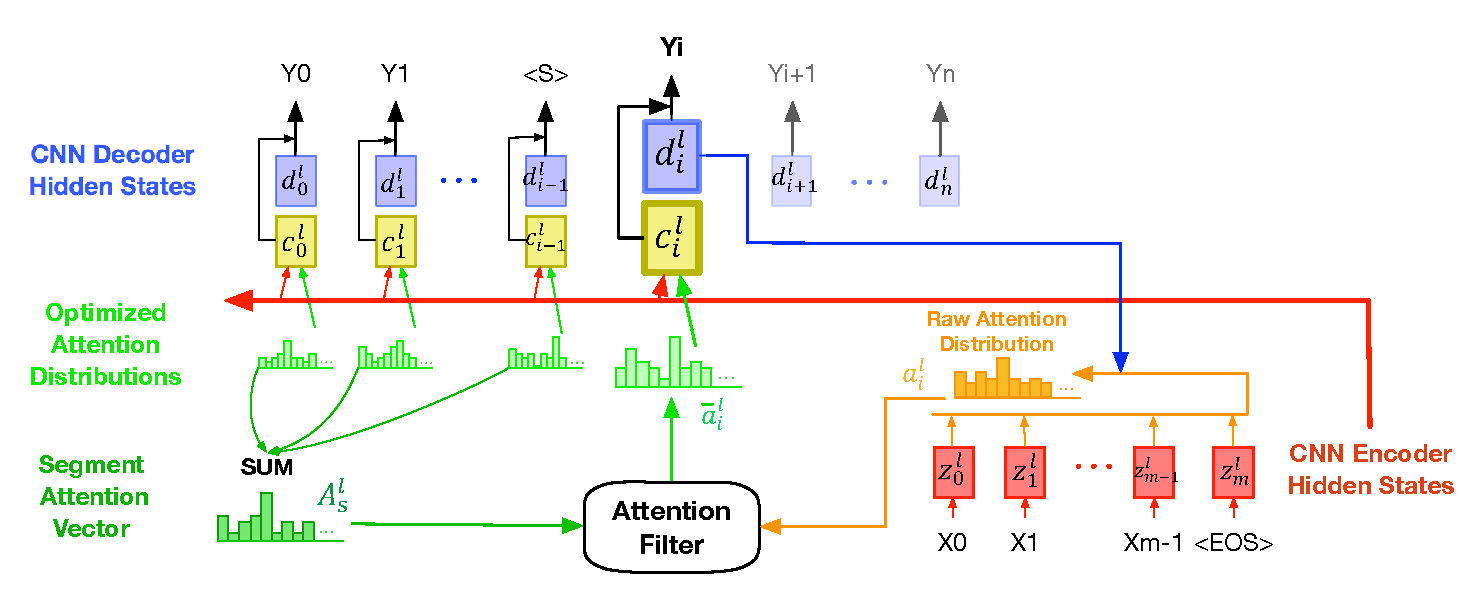
\epsfig{file=model.eps, width=1.0\columnwidth}
	%\caption{Overview of proposed model, which shows how Attention Filter Mechanism (ATTF) works when decoding $Y_i$.}
	\caption{Overview of Attention Filter Mechanism (ATTF)}
	\label{fig:model_main}
\end{figure}


\label{sec:attnf}
%We propose an attention filter mechanism based on basic model
We propose an attention filter mechanism as a novel extension 
to the basic model,
which can record previously attended locations 
%previously POIs 
in the source document directly and generate summaries 
%without repetition
with a natural level of repeatedness. 
This method aims at relieving the repetition problem caused by 
decoders attending to the same POI in source document.

In this mechanism, both source documuent and summary are 
respectively split into 
\textit{sections} and \textit{segments} by punctuations. We
denote the punctuation marks as \verb#<S>#.
$\mathbf{u}=(u_{0},u_{1},...,u_{M})$ 
and $\mathbf{v}=(v_{0},v_{1},...,v_{N})$
denote the positions of \verb#<S># in source document and summary.
Both $u_{0}$ and $v_{0}$ are $-1$.
%Source document $\mathbf{U}=(U_{0},U_{1},...,U_{M-1})$ 
%and summary $\mathbf{V}=(V_{0},V_{1},...,V_{N-1})$ are represented in the form of sections and.
Therefore, we can represent source document as $\mathbf{U}=(U_{0},U_{1},...,U_{M-1})$ in the form of \textit{sections}. Similarly, for summaries, we have $\mathbf{V}=(V_{0},V_{1},...,V_{N-1})$. 
$U_i$ and $V_i$ are
both sequence of tokens minus the punctuation tokens.
%\KW{They are all substrings splitted by punctuations.}

Let $D$ denote the number of tokens in the source document.
We define \textit{segment attention vector} in the $l$-th layer as 
$A^{l} = (A_{0}^{l}, A_{1}^{l},..., A_{N}^{l})$, 
where $A_s^l\subset \mathbb{R}^{D}$ is a vector representing 
segment attention distribution, of the $s$-th \textit{segment},
over tokens in the source document. Summing up attention score vectors 
of each position in the $s$-th \textit{segment}:
%which is the sum of attention distributions over each section in summary:

\begin{equation}
\small
    A_{s}^{l} = \sum_{i=v_{s-1}+1}^{v_{s}-1}a_{i}^{l}
\end{equation}
where $a_i^l$ is also a $D$-dimensional vector that records 
the attention scores of the $i$-th token in the summary over 
tokens in the source document. In other words, $ A_{s}^{l}$ 
measures the relevance between tokens of the source document and 
the $s$-th \textit{segment} $V_s$. 
%where vector $A_{n}^{l}$ is the partial attention distribution over the words in source document. 
%It represents the degree of relevance between source document and the $n$-th section in summary.
We set $A_{0}^{l}$ as zero vector, because nothing is attended before generating 
the first \textit{segment}. 


To find the most attended \textit{sections}, 
we sort the elements inside the filter vector, 
$A_{s}^{l}$, in descending order, 
and record the top $k$ elements' positions in 
the source document as: 
\begin{equation}
\small
    \mathbf{p}=(p_{0},...,p_{k})
\end{equation}
where $k=v_{s}-v_{s-1}-1$.
%To get the attended sections of document, we sort elements $A_{nj}^{l}$ in descending order, and record the positions a
%in decreasing order, and record the position
%$\mathbf{p}=(p_{0},...,p_{k})$, of 
%top $k$ elements in source document, where $k = v_{n} - v_{n-1}$. 
%The higher value of $A_{nj}^{l}$ means that the $j$-th words of source document has been attended. 
%We find out which section of these top $k$ elements belong to by $\mathbf{p}$ and $\mathbf{u}$.
Next, we locate these elements in the source document as well as
the \textit{sections} they belong to. 
We assign each section a set of positions that have been attended to, 
$P_{U_{t}}$. 
If the size of $P_{U_{t}}$ is larger than
$sz$, a predefined constant,
%\footnote{$sz$ is a constant. 
%We set $sz$ as 3, because nearly 90 percent
%of sections with lengt$>=$3.}, 
the \textit{section} $U_{t}$ should not be attended again. 
That is, $U_{t}$ is a POI of segment $V_{s}$.
%We use $\bar{U}$ to express this kind of section. 
$\mathbb{U}_{s}$ denotes a set of all such POIs for $V_s$.
$\mathbb{U}_{0}$ is an empty set.
%the \textit{section $U_{t}$} can be seen as the POI by $V_s^{l}$. 

We construct two multi-hot vectors $g_{s}$ and $g'_{s}$ for each \textit{segment} $V_{s}$.
The dimensions of them are the
same as $A_{s}^{l}$. For $g_{s}$, we set elements on the position of tokens
belonging to sections in $\mathbb{U}_{s}$ to 0, and other
%same as $A_{s}^{l}$. For $g_{s}$, we set elements on the position of POIs to 0, and other
positions to 1. $g'_{s}$ is the flipped version of $g_{s}$. 
%The filter on $a_{ij}^{l}$ in Equation (\ref{eq:a} is to minimize elements of POIs:
The filter on $a_{ij}^{l}$ in Equation (\ref{eq:a}) is given as:
%DIF < \KZ{Can we simplify the notations a bit? What are $A^l_{sj}$ and
%DIF < $g_{sj}'$? We had $A^l_s$ before ... It's a bit confusing.}
%DIF > \begin{equation}
%DIF > \small
%DIF >     e_{s} = \min \limits_{A_{s}}\left(\frac{A_{sj}^{l}}{v_{s}-v_{s-1}-1}\right)
%DIF > \end{equation}
%DIF > \begin{equation}
%DIF > \small
%DIF >     \tilde{a}_{ij}^{l} = a_{ij}^{l}\prod_{q=0}^{s}g_{qj} + e_{s}g_{sj}'
%DIF >     %\bar{a_{ij}}^{l} = a_{ij}^{l}\prod_{q=0}^{n}s_{q} + \min\frac{A_{n}^{l}}{v_{n}-v_{n-1}}t_{n}
%DIF > \end{equation}
\begin{equation}
\small
	\DIFdelbegin \DIFdel{e_{s} }\DIFdelend \DIFaddbegin \tilde{a}\DIFadd{_{ij}^{l} }\DIFaddend = \DIFaddbegin \DIFadd{a_{ij}^{l}\prod_{q=0}^{s}g_{qj} + }\DIFaddend \min \limits_{A_{s}}\left(\frac{A_{sj}^{l}}{v_{s}-v_{s-1}-1}\right)\DIFaddbegin \DIFadd{g_{sj}'
}\DIFaddend \end{equation}
\DIFdelbegin \begin{displaymath}
\DIFdel{\small
    \tilde{a}_{ij}^{l} = a_{ij}^{l}\prod_{q=0}^{s}g_{qj} + e_{s}g_{sj}'
    %DIF < \bar{a_{ij}}^{l} = a_{ij}^{l}\prod_{q=0}^{n}s_{q} + \min\frac{A_{n}^{l}}{v_{n}-v_{n-1}}t_{n}
}\end{displaymath}
%DIFAUXCMD
\DIFdelend where $v_{s}$ is the maximum value in 
$\mathbf{v}$ that is smaller than $i$, and $\tilde{a}_{ij}^l$ is the filtered
attention score. $A_{sj}$ is the attention score between $j$-th token
of the source document and the $s$-th \textit{segment}. 
$g_{sj}$ and $g_{sj}'$ denote whether $j$-th token
of the source document has been attended.
%\XS{Hard to understand this definition of ``n''. And ``n'' is already used to be the size of output in Section 2.1}
Equation (\ref{eq:c}) now becomes:
\begin{equation}
\small
    c _ { i } ^ { l } = \sum _ { j = 1 } ^ { m } \tilde{a}_{ij}^{l} \left( z _ { j } ^ { u } + X_j \right)
\end{equation}

%We pick $K$ sections with highest attention which is calculated by:
%\begin{equation}
%    A_{nj}^{l} = \sum^{P}A_{nj}^{l}
%\end{equation}  

%This method find out the attended location in source document directly and accurately.
%Then it filters out attention of the attended location from the attention distribution. 
%%In this way, our attention filter is capable of comprehending the attention history in a precise and direct manner. 
%The previous approaches revise attention scores
%through decoder hidden state. They can not locate POIs exactly.
%The coverage model which gets the sum of all previous attention can 
%bring attention noise, especially in the long summary.

%Because of using segment attention and revising attention score of attended POIs directly,
By using segment-wise attention and revising attention \DIFdelbegin \DIFdel{score }\DIFdelend \DIFaddbegin \DIFadd{scores }\DIFaddend of attended POIs directly,
%it optimizes the 
%\KW{compared with token-wise attention,}
our model optimizes the
attention distribution between encoder states and decoder states in such a way that
the alignment relationship between source document and summary is enhanced, 
and noise for attention from encoder outputs is reduced. 
As shown in \tabref{tab:attn_exp}, the segments in example are separated by punctuation.
For basic CNN model, the 2nd and 3rd sentence repeatedly attend to 
the 5th segment in source.
After applying ATTF model, 
the attention score of 3rd and 5th segment in source are penalized 
during generating words in 3rd sentence of ATTF.
The last sentence of the summary generated by ATTF attend to 7th segment in source.

\begin{table}[th!]
\begin{center}
\scriptsize
\begin{tabular}{|l|l|}%{|p{7cm}|rl|}
\hline 
\multicolumn{2}{|c|}{\bf Source document} \\
\hline
\multicolumn{2}{|c|}{\tabincell{l}{(1)justin timberlake and jessica biel, (2)welcome to parenthood. 
	   (3)the celebrity couple announced the arrival \\
           of their son, 
           (4)... 
	   (5)the couple announced the pregnancy in january, (6)...  
	   (7)it is the first baby for both . }} \\
\hline 
\bf Basic CNN model (CNN) & \bf ATTF (our) \\
\hline 
\tabincell{l}{(1)the couple announced the the arrival of their son. \\
              (2)the couple announced the pregnancy in january. \\ 
              (3)the couple announced the pregnancy in january. } 
& \tabincell{l}{(1)the couple announced the arrival of their son. \\
	            (2)the couple announced the pregnancy in january. \\
	            (3)it is the first baby for both. } \\
\hline
\end{tabular}
\end{center}
\caption{\label{tab:attn_exp} Summary generated by the basic CNN model and ATTF model}
\end{table}
The attention filter mechanism helps avoid repeatedly attending to the same POIs, and therefore avoid repetition in summary generation.


\subsection{Sentence-level Backtracking Decoder (SBD)}
\DIFaddbegin \label{sec:sbd}
\DIFaddend 

%As mentioned in \secref{sec:intro}, another reason that gives rise to 
%repetition in summaries is repeated sentences or phrases in 
%source documents.
%To handle the repetition caused by repetitive sentences in source document(\tabref{tab:src_rep}),
%To tackle repeated sentences or phrases in the source document (\exref{ex:repeatsrc}), 
%we propose a sentence-level backtracking decoder at testing.
To tackle repeated sentences or phrases in the source (\exref{ex:repeatsrc}), 
we propose a sentence-level backtracking decoder.

\begin{figure}[th]
    \centering
    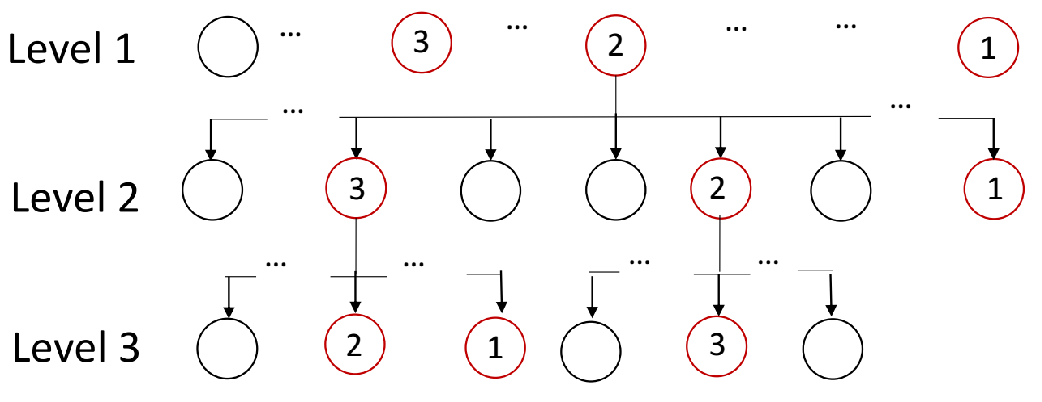
\includegraphics[width=0.8\linewidth]{SBD}
    \caption{Backtracking in Beam Search ($b=3$)\DIFaddbeginFL \DIFaddFL{. 
	    This figure shows the progress of generating summary at test. The circles denote the
		candidate words (choices) in vocabulary, 
		which are sorted by the probability of being selected in
		descending order. Each circle at level $l$ has $N$ choices 
		at level $l+1$. $N$ is the number of words in vocabulary. 
		The number in circles is the order of these choices according to the
		probability. The generation order is from level 1 (top) to level 3 (bottom).}\DIFaddendFL }
    \label{fig:beam}
\end{figure}

At test time, we prevent the decoder from generating identical or
very similar sentences more than once via backtracking. 
An intuitive solution is to backtrack the generation process to the beginning
of the repeated segment, and regenerate it by following the second best choice
in the beam. We call this simple approach \DIFdelbegin \DIFdel{SBD-b1.
}\DIFdelend \DIFaddbegin \textbf{\DIFadd{SBD-b1}}\DIFadd{.
%DIF > However, this is sub-optimal because the parents of the current top $b$
%DIF > choices may not include all the top $b$ choices at the parent level, e.g.,
%DIF > the first choices at level 1 and 2 are excluded by beam search,
%DIF > as shown in \figref{fig:beam}. Here $b$ is the beam size.
}\DIFaddend However, this is sub-optimal
because the parents of the current top $b$ choices may not include all the top $b$ choices at the
parent level\DIFdelbegin \DIFdel{, e. g. }\DIFdelend \DIFaddbegin \DIFadd{. Here $b$ is the beam size. As shown in }\figref{fig:beam}\DIFadd{, suppose that level 3 is the
beginning of the repeated segment}\DIFaddend , the first choices at level 1 and 2 are excluded by beam search\DIFdelbegin \DIFdel{,
as shown in }%DIFDELCMD < \figref{fig:beam}%%%
\DIFdel{. Here $b$ is the beam size. 
}\DIFdelend \DIFaddbegin \DIFadd{. 
%DIF > after generating words based on second and third choices in level 2.
}\DIFaddend 

An alternative approach (\DIFdelbegin \DIFdel{SBD-b2}\DIFdelend \DIFaddbegin \textbf{\DIFadd{SBD-b2}}\DIFaddend ) backtracks all the way until the current
top $b$ choices all share the same prefix token sequence. This means
that the current best choices in the beam reach some consensus that
the generated prefix summary is good and should be retained. 
While this algorithm backtracks further and may
include better choices, it \DIFdelbegin \DIFdel{doesn't }\DIFdelend \DIFaddbegin \DIFadd{does not }\DIFaddend completely solve the problem of SBD-b1. 
\DIFaddbegin \DIFadd{As shown in }\figref{fig:beam}\DIFadd{, 
suppose that level 3 is the beginning of the repeated segment and the second choices in
level 1 is the only prefix token sequence of top $b$ choices in level 2, the first and third choices at
level 1 are excluded by beam search after generating words based on second choice in level 1.
}

\begin{table}[th!]
\begin{center}
\scriptsize
\begin{tabular}{|l|l|}%DIF > {|p{7cm}|rl|}
\hline 
\multicolumn{2}{|c|}{\bf Source document} \\
\hline
\multicolumn{2}{|c|}{\tabincell{l}{
justin timberlake and jessica biel , welcome to parenthood . the celebrity couple announced \\
the arrival of their son , silas randall timberlake ,... `` silas was the middle name of \\
timberlake 's maternal grandfather bill bomar , who died in 2012 ,... the couple announced \\
the pregnancy in january , with an instagram post . it is the first baby for both .
}} \\
\hline 
\bf \DIFaddFL{Basic CNN model (CNN)
}& \tabincell{l}{
				the couple announced the arrival of their son. \\
			    the couple announced the pregnancy in january. \\
				\textit{the couple announced the pregnancy in january. (repeated segment)} \\
				} \\
\hline 
\bf \DIFaddFL{CNN+SBD-b1
}& \tabincell{l}{
				the couple announced the arrival of their son. \\
				the couple announced the pregnancy in january. \\
				\underline{silas was the middle name of timberlake 's maternal grandfather.} \\
				} \\
\hline
\bf \DIFaddFL{CNN+SBD-b2
}& \tabincell{l}{
				the couple announced the arrival of their son. \\
				\underline{silas randall timberlake , died in 2012.} \\
				} \\
\hline
\bf \DIFaddFL{CNN+SBD
}& \tabincell{l}{
				the couple announced the arrival of their son. \\
                they announced the pregnancy in january, with an instagram post. \\
				} \\
\hline
\end{tabular}
\end{center}
\caption{\label{tab:sbd_exp} \DIFaddFL{Summary generated by basic CNN model with different backtracking methods.}}
\end{table}
\DIFaddend 

Our best approach (\DIFdelbegin \DIFdel{SBD}\DIFdelend \DIFaddbegin \textbf{\DIFadd{SBD}}\DIFaddend ) backtracks to the beginning of the whole summary
and regenerates all the choices in the beam up to the point before
the repeated segment. That way, all the best choices are known to the
algorithm and we can make an optimal choice after excluding the first word
of the previously repeated segment. 
%DIF < When regenerating a new summary, 
%DIF < we do not generate the same word as the first word in $S$ at step $p$.
%DIF < our model do not consider the starting word of $S$ at step $p$.
%DIF < Another two versions of backtracking are compared in \secref{sec:eval}.
%DIF < One (SBD-b1) is to regenerate this sentence from the end of last sentence.
%DIF < SBD-b1 only backtracks to the beginning of the last sentence.
%DIF < The other (SBD-b2) is backtracking to the most adjust decoder state 
%DIF < that all of generated sequences in beam size
%DIF < before this state are the same.
%DIF < Whereas SBD-b2 backtracks to the timestamp where all $k$ candidate sequences in beam search are exactly the same, where $k$ denotes beam size. 
%DIF < \KW{not sure if i get it right}
\DIFaddbegin \DIFadd{As shown in }\tabref{tab:sbd_exp}\DIFadd{,
SBD-b1 and SBD-b2 backtrack the generator process
to ``january.'' and ``son.'' respectively.
The summaries generated by SBD-b1 and SBD-b2 
are incoherence and inconsistent with the source document.
Our best approach (SBD) will save the sequence before repeated segment, i.e., 
`}\textit{
\DIFadd{the couple announced the arrival of their son.
the couple announced the pregnancy in january.}}
\DIFadd{'
and backtrack to the beginning of the summary and regenerate the summary. 
When the saved sequence appears in the beam, we remove the first word (``the'') in 
repeated segment from the choices vocabulary. 
Compared with SBD-b1 and SBD-b2, SBD generates more fluent and coherence summaries.
}\DIFaddend 


To determine whether two sentences, 
$p$ and $q$, are similar, we define a boolean function as:
%DIF > \begin{equation}\label{eq:s}
%DIF > \small
%DIF >     sim(p,q) = o > n\text{ OR }o > \frac{1}{2}\cdot l
%DIF > \end{equation}
%DIF > where $o$ denotes the length of the longest common substring (LCS) between $p$ and $q$, 
%DIF > $l$ is the minimum of the lengths of $p$ and $q$, and $n$ is a constant. 
%DIF > $sim(p,q)=1$ means the two sentence are similar.
\begin{equation}\label{eq:s}
\small
	sim(p,q) = 
	\DIFdelbegin \DIFdel{o > n\text{ OR }o > \frac{1}{2}\cdot l
}\DIFdelend \DIFaddbegin \begin{cases}
		   1 &\mbox{if $o(p,q) > n\text{ OR }o(p,q) > \frac{1}{2}\cdot l$}\\
		   0 &\mbox{others}
   \end{cases}
\DIFaddend \end{equation}
where \DIFdelbegin \DIFdel{$o$ }\DIFdelend \DIFaddbegin \DIFadd{$o(p,q)$ }\DIFaddend denotes the length of 
the longest common substring (LCS) between $p$ and $q$, 
$l$ is the minimum of the lengths of $p$ and $q$, and $n$ is a constant. 
$sim(p,q)=1$ means the two sentence are similar.
%DIF < We set $n$ as 5, because the number of overlapped words in target summaries
%DIF < is less than 5 percent.
%DIF < \KW{maybe mention c=5 in experiment settings, the notation in the formula is not clean enough but i don't know how to revise it}

%DIF < This method does not attempt to impact the process of beam search in the middle of a sentence so that we are free of grammatical and factual errors compared with our \textbf{TRI} baseline.
This method cooperates with ATTF in 
reducing repetition caused by the noises in the dataset.
It does not interrupt the beam search process in the middle of a sentence, 
hence significantly reducing related grammatical and factual errors 
compared with \textbf{TRI}.
%which we validate in \tabref{tab:strong_methods}.
Besides, it is capable of producing a more informative summary since
it yields more chances to other candidate sentences.
%, which we validate in relevant experiments
%(\tabref{tab:src_rep}, \figref{fig:attn_map3}).

\section{Evaluation}
\label{sec:eval}
%DIF < In this section, we introduce the experimental setup
%DIF < and analyze the performance of different models.
%DIF < All of the data and source code
%DIF < can be downloaded from http://202.120.38.146/sumrep.}.
\DIFaddbegin \DIFadd{In this section, we introduce the experimental setup
and analyze the performance of different models.
}\DIFaddend 

\subsection{Datasets}
CNN/Daily Mail~\cite{HermannKGEKSB15}
\footnote{\url{https://cs.nyu.edu/~kcho/DMQA/}} 
is a popular summarization dataset, 
which contains news articles paired with summaries.
There are 286,817 training pairs,
13,368 validation pairs and 11,487 test pairs.
\tabref{tab:example} shows an example pair from training data.
We follow See~\cite{SeeLM17} in data preprocessing and use 
the non-anonymized version, which fills in the blanks with answer named entities.
%DIF < We show an example of such pairs in \tabref{tab:gold_a}.


\subsection{Model Parameters and Evaluation Metrics}
\label{sec:expset}
All the competing models contain $8$ convolutional layers in
both encoders and decoders, with kernel width of $3$.
For each convolutional layer, 
we set the hidden state size to $512$ and the embedding size to $256$.
%DIF < To alleviate overfitting,
\DIFdelbegin \DIFdel{We }\DIFdelend \DIFaddbegin \DIFadd{To alleviate overfitting,
we }\DIFaddend apply a \textit{dropout} ($p=0.2$) layer to 
all convolutional and fully connected layers.
Similar to \cite{gehring2017convs2s},we use Nesterov's
accelerated gradient method \cite{SutskeverMDH13} with gradient clipping $0.1$ \cite{PascanuMB13}, momentum $0.99$,
%DIF < accelerated gradient method with gradient clipping $0.1$, momentum $0.99$,
and initial learning rate $0.2$.
Training terminates when learning rate $\le 10e$-$5$.
Beam size $b=5$ at test time.

We set the threshold $sz$ to $3$, 
because nearly $90\%$ 
of sections are with length$>=$3.
We set $n$ (Equation (\ref{eq:s})) to $5$,
since less than $5\%$ of reference summaries have
the LCS of less than $5$.
We use the following evaluation metrics:
\itemsep0em
\begin{itemize}

\item \textbf{ROUGE} scores (F1), including ROUGE-1 (R-1), ROUGE-2 (R-2) and
ROUGE-L(R-L)~\cite{rouge-a-package-for-automatic-evaluation-of-summaries}.
%DIF < ROUGE-2 is the most popular metric for summarization.
\DIFaddbegin \DIFadd{ROUGE-2 is the most popular metric for summarization.
}\DIFaddend 

\item \textbf{Repeatedness} (Rep) 
includes N-gram repeatedness, sentence repeatedness
and total repeatedness.
\DIFdelbegin \DIFdel{N-gram or sentence repeatedness }\DIFdelend \DIFaddbegin \begin{itemize}
\item[-] \textbf{\DIFadd{N-gram repeatedness}} \DIFaddend is the percentage of repeated N-grams 
\DIFdelbegin \DIFdel{or sentences }\DIFdelend in a summary:

\begin{equation}
\small Rep\DIFaddbegin \DIFadd{_{ngram} }\DIFaddend = \DIFdelbegin \DIFdel{\frac{n}{N}
}\DIFdelend \DIFaddbegin \DIFadd{\frac{n_{ngram}}{N_{ngram}}
}\DIFaddend \end{equation}
where \DIFdelbegin \DIFdel{$n$ }\DIFdelend \DIFaddbegin \DIFadd{$n_{ngram}$ }\DIFaddend is the number of repeated N-grams\DIFdelbegin \DIFdel{or sentences, 
$N$ }\DIFdelend \DIFaddbegin \DIFadd{, 
$N_{ngram}$ }\DIFaddend is the total number of N-grams \DIFdelbegin \DIFdel{or sentences }\DIFdelend in a summary.
\DIFdelbegin \DIFdel{We use }\textit{\DIFdel{sim}} %DIFAUXCMD
\DIFdel{in }%DIFDELCMD < \eqnref{eq:s} %%%
\DIFdel{to
%DIF < estimate whether an N-gram or a sentence repeats.
identify repetitive sentences.
Total repeatedness}\DIFdelend \DIFaddbegin \item[-] \textbf{\DIFadd{Sentence repeatedness}} \DIFadd{is the percentage of repeated 
sentences in a summary:
}\begin{equation}
\DIFadd{\small Rep_{sent} = \frac{n_{sent}}{N_{sent}}
}\end{equation}
\DIFadd{where $n_{sent}$ is the number of repeated sentences, 
$N_{sent}$ is the total number of sentences in a summary.
For sentence repeatedness, if the sentences contain the same trigram,
these sentence are repetitve sentences.
}\footnote{
\DIFadd{Any two sentences in one reference summary almost never contain 
the same trigram \mbox{%DIFAUXCMD
\cite{PaulusXS17}}\hspace{0pt}%DIFAUXCMD
.}}
\item[-] 
\textbf{\DIFadd{Total repeatedness}} \DIFaddend (Algorithm \ref{alg:red}) is a comprehensive score
that unifies \DIFaddbegin \DIFadd{word-level and sentence-level repeatedness.
It is not computed by }\DIFaddend N-gram \DIFaddbegin \DIFadd{repeatedness score 
}\DIFaddend and sentence repeatedness \DIFaddbegin \DIFadd{score}\DIFaddend .

\begin{algorithm}[th]
\caption{Calculation of Total Repeatedness}
\small
\label{alg:red}
\textbf{Input}: a sentence set $s = {s_{1}, s_{2},...,s_{n}}$\\
%\textbf{Parameter}: Optional list of parameters\\
\textbf{Output}: Total repeatedness percentage $p$
\begin{algorithmic}[1] %[1] enables line numbers
\STATE Let $total$ be the sum of lengths of the sentences in $s$.
\STATE $n \leftarrow total$
\STATE $overlap \leftarrow 0$
\WHILE{$n \geq 3$}
\STATE The lengths of LCS between two sentences from $s$ comprise a length set $L$.
\STATE $n \leftarrow \max(L)$.
\STATE Find a substring $b$ with length $n$ that appears most frequently in $s$.
\STATE Let $k$ be the frequency that $b$ appears in $s$.
\STATE $overlap \leftarrow overlap + k\cdot n$
\STATE Remove every appearance of substring $b$ from sentences in $s$.
\ENDWHILE
\STATE $p \leftarrow overlap/total$
\STATE \textbf{return $p$} 
\end{algorithmic}
\end{algorithm}
\DIFaddbegin \end{itemize}
\DIFaddend 

\item \textbf{\DIFdelbegin \DIFdel{Readability}%DIFDELCMD < } %%%
\DIFdel{(Readable)is human evaluation,
the percentage of }\textit{\DIFdel{readable}} %DIFAUXCMD
\DIFdel{sentences in summaries.
%DIF < Sentences are more complete than segment so that they can
%DIF < be evaluated easily.
Here we score sentences instead of segments because segments often have
insufficient information to determine readability.
A }\textit{\DIFdel{readable}} %DIFAUXCMD
\DIFdel{sentence is free of grammatical and factual errors, }\DIFdelend \DIFaddbegin \DIFadd{Repeatedness Correlation}} 
\DIFadd{measures test how well 
the total repeatedness scores of summaries generated by each model
correlate with total repeatedness scores of reference summaries. 
The more correlative generated summary and reference summary are,
the better generated summary is.
The correlation is evaluated with a set of
three metrics, including Pearson correlation (r),
Spearman rank coefficient ($\rho$), and Kendall's tau coefficient ($\tau$).
Given total repeatedness scores of reference summaries (ref) and 
their corresponding generated summaries (gen),
$X=score(ref)=(x_1, x_2,..., x_n)$ }\DIFaddend and 
\DIFdelbegin \DIFdel{is }\DIFdelend \DIFaddbegin \DIFadd{$Y=score(gen)=(y_1, y_2,..., y_n)$, 
we can get paired data $(X,Y)={(x_1, y_1), (x_2, y_2),..., (x_n, y_n)}$.
$n$ is the number of pairs.
}\begin{itemize}	
\item[-] \DIFadd{For Pearson correlation (r),
}\begin{equation}
\DIFadd{r = \frac{\sum_{i=1}^{n}(x_i - \overline{X})(y_i - \overline{Y})}{\sqrt{\sum_{i=1}^{n}(x_i - \overline{X})^{2}\cdot\sum_{i=1}^{n}(y_i - \overline{Y})^{2}}}
}\end{equation}
\DIFadd{where $\overline{X}$ and $\overline{Y}$ are the mean of variables of $X$ and $Y$.
}

\item[-] \DIFadd{For Spearman rank coefficient,
}\begin{equation}
\DIFadd{\rho = \frac{\sum_{i=1}^{n}(R(x_i) - \overline{R(X)})(R(y_i) - \overline{R(Y)})}{\sqrt{\sum_{i=1}^{n}(R(x_i) - \overline{R(X)})^{2}
	  \cdot\sum_{i=1}^{n}(R(y_i)-\overline{R(Y)})^{2}}}
}\end{equation}
\DIFadd{where $R(x_i)$ and $R(y_i)$ are the rank of $x_i$ and $y_i$.
$\overline{R(X)}$ and $\overline{R(Y)}$ are the mean rank of $X$ and $Y$.
}

\item[-] \DIFadd{For kendall's tau coefficient,
}\begin{equation}
\DIFadd{\tau = \frac{n_c - n_d}{n_c + n_d} = \frac{n_c - n_d}{n(n-1)/2}
}\end{equation}
\DIFadd{where $n_c$ is the number of }\textit{\DIFadd{concordant}} \DIFadd{pairs.
$n_d$ is the number of }\textit{\DIFadd{discordant}} \DIFadd{pairs.
Any pair of total repeatedness scores $(x_{i},y_{i})$ and $(x_{j},y_{j})$, where $i<j$.
They are said to be }\textit{\DIFadd{concordant}}\DIFadd{,
if both $x_{i}>x_{j}$ and $y_{i}>y_{j}$; or if both $x_{i}<x_{j}$ and $y_{i}<y_{j}$.
They are said to be discordant, if $x_{i}>x_{j}$ and $y_{i}<y_{j}$; 
or if $x_{i}<x_{j}$ and $y_{i}>y_{j}$. 
If $x_{i}=x_{j}$ or $y_{i}=y_{j}$, the pair is neither concordant nor discordant.
}\end{itemize}


\item \textbf{\DIFadd{Readability}} \DIFadd{(Readable) is a human evaluation. 
We educate human annotators to assess each summary
from three independent perspectives: 
(1) Informative: How informative the summary is? 
Is the summary }\DIFaddend logically consistent with source document\DIFdelbegin \DIFdel{.
%DIF < \begin{equation}
%DIF < Correct = \frac{n_{ct}}{N_{all}}
%DIF < \end{equation}
%DIF < where $n_{ct}$ and $N_{all}$ denotes
%DIF < the number of \textit{correct} sentences and all sentences 
%DIF < in a summary respectively.
}\DIFdelend \DIFaddbegin \DIFadd{? 
(2) Coherent: How coherent (between sentences) the summary is? 
(3) Fluent: How grammatical the sentences of a summary are? 
Are there any factual errors in the summary?
Readability score will be judged on the following 5-point scale:
Very Poor (1.0), Poor (2.0), Barely Acceptable (3.0), Good (4.0) and Very Good (5.0).
The score reflects the fluency and readability of the summary.
}\DIFaddend \end{itemize}

We use \textit{readability} to complement ROUGE scores 
since Yao~\cite{YaoWX17} showed that the standard 
ROUGE scores cannot capture grammatical or factual errors. 
We randomly sample 300 summaries generated by each model
and manually check their readability. 
%DIF < This is a simplified human-evaluation of summarization,  
%DIF < It is easier to do and more reliable than other human-evaluations
%DIF < since we only need to check whether the sentences in a summary are \textit{correct} or not.
\DIFdelbegin \DIFdel{This metric is more objective and practical compared with
scoring the whole summary \mbox{%DIFAUXCMD
\cite{D18-1205}}\hspace{0pt}%DIFAUXCMD
, since we only need 
to determine whether a sentence is }%DIFDELCMD < {\em %%%
\DIFdel{readable}%DIFDELCMD < } %%%
\DIFdel{or not.
Each sentence }\DIFdelend \DIFaddbegin \DIFadd{Each summary }\DIFaddend is scored by two judges proficient in English. 
The Cohen's Kappa coefficient between them is \DIFdelbegin \DIFdel{$0.83$}\DIFdelend \DIFaddbegin \DIFadd{$0.78$}\DIFaddend , 
indicating agreement. Here we use the average annotation score.
%DIF < The score of each model is the proportion
%DIF < of {\em readable} sentences in total.

\subsection{Baselines}
%DIF < In this experiment, we take vanilla CNN seq2seq model as our basic model,
\DIFdelbegin \DIFdel{We take }\DIFdelend \DIFaddbegin \DIFadd{Our goal is to evaluate the
effectiveness of our repetition reduction technique.
We choose to implement 
all existing repetition reduction techniques (}\tabref{tab:baselines}\DIFadd{) 
on top of vanilla CNN seq2seq model.
}

\begin{table}[th]
	\centering
	\small
	\begin{tabular}{|l|l|}
		\hline
		\textbf{\DIFaddFL{Abbrev.}} & \textbf{\DIFaddFL{Description}} \\ \hline
		\textbf{\DIFaddFL{CNN}} &  \DIFaddFL{Convolutional seq2seq model~\mbox{%DIFAUXCMD
\cite{gehring2017convs2s} }\hspace{0pt}%DIFAUXCMD
}\\
		\hline
		\textbf{\DIFaddFL{ITA}} &  \DIFaddFL{Intra-temporal attention~\mbox{%DIFAUXCMD
\cite{NallapatiZSGX16} }\hspace{0pt}%DIFAUXCMD
}\\
		\hline
	%DIF > 	\textbf{ITDA} & \tabincell{l}{Intra-temporal attention and intra-decoder attention\\ \cite{PaulusXS17,FanGA18}}\\
		\textbf{\DIFaddFL{ITDA}} & \tabincell{l}{Intra-temporal attention and intra-decoder attention~\cite{PaulusXS17,FanGA18}}\\
		\hline
	    \textbf{\DIFaddFL{COV}}	& \DIFaddFL{Coverage mechanism~\mbox{%DIFAUXCMD
\cite{SeeLM17}}\hspace{0pt}%DIFAUXCMD
}\\
		\hline
	    \textbf{\DIFaddFL{COVP}}	& \DIFaddFL{Coverage penalty~\mbox{%DIFAUXCMD
\cite{GehrmannDR18}}\hspace{0pt}%DIFAUXCMD
}\\
		\hline
	    \textbf{\DIFaddFL{SCL}}	& \DIFaddFL{Semantic cohesion loss~\mbox{%DIFAUXCMD
\cite{elikyilmazBHC18}}\hspace{0pt}%DIFAUXCMD
}\\
		\hline
        \textbf{\DIFaddFL{TRI}} & \DIFaddFL{Trigram decoder~\mbox{%DIFAUXCMD
\cite{PaulusXS17} }\hspace{0pt}%DIFAUXCMD
}\\
		\hline
	\end{tabular}
	\caption{\DIFaddFL{Baselines}}
	\label{tab:baselines}
\end{table}

\DIFadd{We take the }\DIFaddend vanilla CNN seq2seq model as our basic model \DIFdelbegin \DIFdel{,
%DIF < because it is a more powerful toolkit for sequence modeling than
%DIF < recurrent seq2seq models~\cite{bai2018empirical}.
}\DIFdelend \DIFaddbegin \DIFadd{to improve on,
}\DIFaddend because it is fast and enjoys the best accuracy among
the other vanilla RNN seq2seq models \DIFaddbegin \DIFadd{such as 
RNN seq2seq model and LSTM seq2seq model.}\DIFaddend ~\cite{bai2018empirical,gehring2017convs2s}.
We did not implement the repetition reduction methods 
on top of SOTA seq2seq models,
because the tricks employed in these SOTA models may 
interact with the repetition reduction methods 
and impact the evaluation results (ROUGE), which complicate the analysis.
\DIFdelbegin \DIFdel{Our }\DIFdelend \DIFaddbegin 

\begin{table}[th!]
\begin{center}
\scriptsize
\subtable[Source document and reference summary]{
  \label{tab:a}
  \begin{tabular}{|l|}%{|p{7cm}|rl|}
  \hline 
  \textbf{Source} \\
  \hline 
  justin timberlake and jessica biel, welcome to parenthood. \\
  the celebrity couple announced the arrival of their son, silas randall timberlake, ... \\
  the couple announced the pregnancy in january, ... it is the first baby for both .  \\
  \hline 
  \textbf{Reference} \\
  \hline 
  timberlake and jessica biel welcome son silas randall timberlake. \\
  the couple announced the pregnancy in january . \\
  \hline
  \end{tabular}
}
\qquad
\subtable[The generaged summaries of source in (a) and their ROUGE score]{
  \label{tab:b}
  \begin{tabular}{|c|l|c|}%{|p{7cm}|rl|}
  \hline \bf model & \bf summary & \bf R-2 \\
  \hline \textbf{COV} & \tabincell{l}{timberlake and jessica biel announced the pregnancy in january. \\
       the couple announced the pregnancy in january.} & 0.60 \\
  \hline \textbf{ATTF+SBD} & \tabincell{l}{the couple announced the arrival of their son, silas randall timberlake. \\
       the couple announced the pregnancy in january. \\ it is the first baby for both.} & 0.52 \\
  \hline
  \end{tabular}
}
\caption{\DIFaddFL{Example of generated summaries}}
\label{tab:compete_exp}
\end{center}
\end{table}
\DIFadd{As shown in }\tabref{tab:compete_exp}\DIFadd{, 
the effectiveness of the repetition reduction is not necessarily
reflected in the ROUGE~\mbox{%DIFAUXCMD
\cite{SeeLM17, PaulusXS17, FanGA18}}\hspace{0pt}%DIFAUXCMD
.
After reducing repetition, the summary becomes better
but the ROUGE score is not improved. 
Therefore our }\DIFaddend evaluation mainly compares 
the effectiveness of different repetition reduction techniques
\DIFdelbegin \DIFdel{,
}\DIFdelend in terms of all \DIFdelbegin \DIFdel{three }\DIFdelend \DIFaddbegin \DIFadd{four }\DIFaddend metrics above. 
If these \DIFaddbegin \DIFadd{repetition reduction }\DIFaddend methods 
were applied on top of more advanced models such as PtGen 
\DIFdelbegin \DIFdel{(effectively it is CNN with mechanism that cannot reduce repetition)}\DIFdelend \DIFaddbegin \DIFadd{~}\footnote{\DIFadd{Effectively it is CNN with mechanism that cannot reduce repetition.}}\DIFaddend , 
the room for improvement on the ROUGE score will be
very limited because the advanced models already achieves very high ROUGE scores for any abstractive
summarization techniques. 
Consequently, the differences in ROUGE scores by these repetition reduction techniques will be
indistinguishable. 
\DIFdelbegin \DIFdel{As shown in }%DIFDELCMD < \tabref{tab:compete_exp}%%%
\DIFdel{, after reducing repetition, the summary becomes better
but the ROUGE score is not improved. 
}\DIFdelend Hence, in this work, 
we \DIFdelbegin \DIFdel{choose to implement these methods (}%DIFDELCMD < \tabref{tab:eval_main}%%%
\DIFdel{) on top of vanilla CNN model.
We }\DIFdelend construct seven baselines %DIF < by converting some of RNN-based models to
%DIF < CNN seq2seq architectures, 
\DIFaddbegin \DIFadd{(}\tabref{tab:baselines}\DIFadd{)
}\DIFaddend by converting
repetition reduction techniques developed on RNN seq2seq models to their
counterparts on CNN seq2seq models,
%DIF < \KZ{How can u convert RNN models to CNN models? I think what you mean is
%DIF < repetition reduction techniques developed on RNN models to their counterparts on CNN models.} 
to be fair.
%DIF < Details are illustrated in Introduction. 
%DIF < \KZ{Not sure what you mean by
%DIF < illustrated in Introduction... It's a bit weird to refer back to previous 
%DIF < sections.}
\DIFdelbegin %DIFDELCMD < 

%DIFDELCMD < \begin{table}[th]
%DIFDELCMD < 	\centering
%DIFDELCMD < 	\small
%DIFDELCMD < 	\begin{tabular}{|l|l|}
%DIFDELCMD < 		\hline
%DIFDELCMD < 		%%%
\textbf{\DIFdelFL{Abbrev.}} %DIFAUXCMD
%DIFDELCMD < & %%%
\textbf{\DIFdelFL{Description}} %DIFAUXCMD
%DIFDELCMD < \\ \hline
%DIFDELCMD < 		%%%
\textbf{\DIFdelFL{CNN}} %DIFAUXCMD
%DIFDELCMD < &  %%%
\DIFdelFL{Convolutional seq2seq model~\mbox{%DIFAUXCMD
\cite{gehring2017convs2s} }\hspace{0pt}%DIFAUXCMD
}%DIFDELCMD < \\
%DIFDELCMD < 		\hline
%DIFDELCMD < 		%%%
\textbf{\DIFdelFL{ITA}} %DIFAUXCMD
%DIFDELCMD < &  %%%
\DIFdelFL{Intra-temporal attention~\mbox{%DIFAUXCMD
\cite{NallapatiZSGX16} }\hspace{0pt}%DIFAUXCMD
}%DIFDELCMD < \\
%DIFDELCMD < 		\hline
%DIFDELCMD < 	%%%
%DIF < 	\textbf{ITDA} & \tabincell{l}{Intra-temporal attention and intra-decoder attention\\ \cite{PaulusXS17,FanGA18}}\\
		\textbf{\DIFdelFL{ITDA}} %DIFAUXCMD
%DIFDELCMD < & \tabincell{l}{Intra-temporal attention and intra-decoder attention~\cite{PaulusXS17,FanGA18}}\\
%DIFDELCMD < 		\hline
%DIFDELCMD < 	    %%%
\textbf{\DIFdelFL{COV}}	%DIFAUXCMD
%DIFDELCMD < & %%%
\DIFdelFL{Coverage mechanism~\mbox{%DIFAUXCMD
\cite{SeeLM17}}\hspace{0pt}%DIFAUXCMD
}%DIFDELCMD < \\
%DIFDELCMD < 		\hline
%DIFDELCMD < 	    %%%
\textbf{\DIFdelFL{COVP}}	%DIFAUXCMD
%DIFDELCMD < & %%%
\DIFdelFL{Coverage penalty~\mbox{%DIFAUXCMD
\cite{GehrmannDR18}}\hspace{0pt}%DIFAUXCMD
}%DIFDELCMD < \\
%DIFDELCMD < 		\hline
%DIFDELCMD < 	    %%%
\textbf{\DIFdelFL{SCL}}	%DIFAUXCMD
%DIFDELCMD < & %%%
\DIFdelFL{Semantic cohesion loss~\mbox{%DIFAUXCMD
\cite{elikyilmazBHC18}}\hspace{0pt}%DIFAUXCMD
}%DIFDELCMD < \\
%DIFDELCMD < 		\hline
%DIFDELCMD <         %%%
\textbf{\DIFdelFL{TRI}} %DIFAUXCMD
%DIFDELCMD < & %%%
\DIFdelFL{Trigram decoder~\mbox{%DIFAUXCMD
\cite{PaulusXS17} }\hspace{0pt}%DIFAUXCMD
}%DIFDELCMD < \\
%DIFDELCMD < 		\hline
%DIFDELCMD < 	\end{tabular}
%DIFDELCMD < 	%%%
%DIFDELCMD < \caption{%
{%DIFAUXCMD
\DIFdelFL{Baselines}}
	%DIFAUXCMD
%DIFDELCMD < \label{tab:baselines}
%DIFDELCMD < \end{table}
%DIFDELCMD < %%%
\DIFdelend 

\subsection{Results}
\label{sec:result}

\textbf{Accuracy.} As shown in \tabref{tab:eval_main}, 
our model (ATTF+SBD) outperforms all the baselines in ROUGE score, 
indicating we are able to generate more
accurate summaries. 

\cut{%%%%%%%%%%%%%
\begin{table}[th]
	\centering
	\small
	\begin{tabular}{|l|c|c|c|}
		\hline
		Model &   R-1 & R-2 & R-L \\
		\hline
		CNN &  34.33 & 14.25 & 35.68 \\
		ITA &  34.30 & 14.20 & 35.67 \\
		ITDA & 34.62 & 14.52 &  35.94 \\
	    COV	& 35.85 & 14.81 &  35.96 \\
	    COVP & 34.53 & 14.41 &  35.81 \\
	    SCL	& 35.13 & 14.61 & 35.93 \\
		ATTF & \bf 36.32 & \bf 15.08 & \bf 36.09 \\
		\hline
		SBD-b1* & 34.24 & 14.33 & 34.75 \\
		SBD-b2* & 35.88 & 14.83 & 35.15 \\
		SBD* & 37.19 & 15.45 & 36.03 \\
        TRI* & 36.81 & 15.47 & 36.00 \\
		ATTF+TRI* & 37.33 & 15.65 & 36.30 \\
		ATTF+SBD* & \bf 37.69 & \bf 15.82 & \bf 36.47 \\
		\hline
	\end{tabular}
	\caption{ROUGE scores on CNN/Daily Mail dataset. `*' denotes 
models with operations during testing.}
	\label{tab:eval_main}
\end{table}
}%%%%%%%%%%%%%
\begin{table}[th!]
\begin{center}
\small
\subtable[The models without operations at test.]{
	    \begin{tabular}{|l|c|c|c|}
		\hline
		Model &   R-1 & R-2 & R-L \\
		\hline
		CNN &  34.33 & 14.25 & 35.68 \\
		ITA &  34.30 & 14.20 & 35.67 \\
		ITDA & 34.62 & 14.52 &  35.94 \\
	    COV	& 35.85 & 14.81 &  35.96 \\
	    COVP & 34.53 & 14.41 &  35.81 \\
	    SCL	& 35.13 & 14.61 & 35.93 \\
		ATTF & \bf 36.32 & \bf 15.08 & \bf 36.09 \\
		\hline
	    \end{tabular}
        }
\qquad
\subtable[The models with operations at test.]{
        %\begin{tabular}{lcccccccc}
	    \begin{tabular}{|l|c|c|c|}
		\hline
		Model &   R-1 & R-2 & R-L \\
		\hline
		SBD-b1* & 34.24 & 14.33 & 34.75 \\
		SBD-b2* & 35.88 & 14.83 & 35.15 \\
		SBD* & 37.19 & 15.45 & 36.03 \\
        TRI* & 36.81 & 15.47 & 36.00 \\
		ATTF+TRI* & 37.33 & 15.65 & 36.30 \\
		ATTF+SBD* & \bf 37.69 & \bf 15.82 & \bf 36.47 \\
		\hline
	    \end{tabular}
        }
\caption{ROUGE scores on CNN/Daily Mail dataset.}
\label{tab:eval_main}
\end{center}
\end{table}


\DIFdelbegin %DIFDELCMD < \begin{table}[th!]
%DIFDELCMD < \begin{center}
%DIFDELCMD < \scriptsize
%DIFDELCMD < \subtable[Source document and reference summary]{
%DIFDELCMD <   %DIFDELCMD < \label{tab:a}%%%
%DIFDELCMD <   \begin{tabular}{|l|}%{|p{7cm}|rl|}
%DIFDELCMD <   \hline 
%DIFDELCMD <   \textbf{Source} \\
%DIFDELCMD <   \hline 
%DIFDELCMD <   justin timberlake and jessica biel, welcome to parenthood. \\
%DIFDELCMD <   the celebrity couple announced the arrival of their son, silas randall timberlake, ... \\
%DIFDELCMD <   the couple announced the pregnancy in january, ... it is the first baby for both .  \\
%DIFDELCMD <   \hline 
%DIFDELCMD <   \textbf{Reference} \\
%DIFDELCMD <   \hline 
%DIFDELCMD <   timberlake and jessica biel welcome son silas randall timberlake. \\
%DIFDELCMD <   the couple announced the pregnancy in january . \\
%DIFDELCMD <   \hline
%DIFDELCMD <   \end{tabular}
%DIFDELCMD < }
%DIFDELCMD < \qquad
%DIFDELCMD < \subtable[The generaged summaries of source in (a) and their ROUGE score]{
%DIFDELCMD <   %DIFDELCMD < \label{tab:b}%%%
%DIFDELCMD <   \begin{tabular}{|c|l|c|}%{|p{7cm}|rl|}
%DIFDELCMD <   \hline \bf model & \bf summary & \bf R-2 \\
%DIFDELCMD <   \hline \textbf{COV} & \tabincell{l}{timberlake and jessica biel announced the pregnancy in january. \\
%DIFDELCMD <        the couple announced the pregnancy in january.} & 0.60 \\
%DIFDELCMD <   \hline \textbf{ATTF+SBD} & \tabincell{l}{the couple announced the arrival of their son, silas randall timberlake. \\
%DIFDELCMD <        the couple announced the pregnancy in january. \\ it is the first baby for both.} & 0.52 \\
%DIFDELCMD <   \hline
%DIFDELCMD <   \end{tabular}
%DIFDELCMD < }
%DIFDELCMD < %%%
%DIFDELCMD < \caption{%
{%DIFAUXCMD
\DIFdelFL{Example of generated summaries}}
%DIFAUXCMD
%DIFDELCMD < \label{tab:compete_exp}
%DIFDELCMD < \end{center}
%DIFDELCMD < \end{table}
%DIFDELCMD < 

%DIFDELCMD < %%%
\DIFdelend Without any special operations at testing, 
our ATTF model achieves the highest ROUGE score, showing
its effectiveness in improving summary quality.
%ATTF is effective to improve the summarization quality of basic CNN seq2seq models.
Models with SBD or TRI at testing
are more effective than the basic CNN seq2seq model,
because more information is involved in summary generation 
as a by-product of repetition reduction.
Compared with its two variants, SBD is a little slower 
but has a higher ROUGE score, reflecting its advantage due to
better choices taken globally.
Therefore, 
we use SBD as our backtracking decoder in the following experiments. 
The number of explored candidate hypothesis, up to a point of
repetition, is less than 30 tokens.
The ROUGE score of SBD is higher than TRI on R-1 and R-L, but lower on R-2. 
The reason is that R-2 and R-L respectively evaluate
bigram-overlap and longest common sequence between the reference
summary and generated summary. This is in line with different techniques 
in SBD and TRI, the former promoting the diversity of sentences and 
the latter promoting that of trigrams.
SBD has higher ROUGE scores than ATTF, 
because the summaries from
SBD do not have the repetition caused by attending to similar sentences in source.
Unlike ATTF, 
SBD cannot obtain the ability to attend to different POIs through training.
In \tabref{tab:src_rep}, the sentences in SBD are not repetitive, 
but summarized from the same POI.
The summaries may lose important information when only using SBD.
The readability score of SBD is lower than ATTF in \tabref{tab:eval_repe}.

\begin{table}[th!]
\begin{center}
\small
\DIFdelbeginFL %DIFDELCMD < \subtable[The models without operations at test.]{
%DIFDELCMD <             \begin{tabular}{|c|c|ccccccc|}
%DIFDELCMD <                 \hline
%DIFDELCMD <                     & Gold & CNN  & ITA & ITDA & COV & COVP & SCL & ATTF \\
%DIFDELCMD <                 \hline
%DIFDELCMD <                 1-gram & 33.79 & 56.25 & 54.44 & 51.18 & 42.18 & 52.46 & 52.23 & \bf 34.98 \\
%DIFDELCMD <                 2-gram & 2.98 & 36.55 & 34.76 & 30.64 & 16.77 & 32.11 & 34.08 & \bf 8.16 \\
%DIFDELCMD <                 3-gram & 0.43 & 32.62 & 31.10 & 27.14 & 12.95 & 28.59 & 30.58 & \bf 5.11 \\
%DIFDELCMD <                 4-gram & 0.12 & 30.18 & 28.85 & 25.04 & 11.17 & 26.48 & 28.34 & \bf 4.19 \\
%DIFDELCMD <                 Sent & 0.08 & 37.04 & 35.79 & 31.46 & 13.98 & 24.63 & 26.38 & \bf 3.56 \\
%DIFDELCMD <                 \hline
%DIFDELCMD <                 Total-Rep & 0.51 & 18.86 & 17.94 & 15.62 & 7.77 & 16.46 & 17.65 & \bf 3.27 \\
%DIFDELCMD <                 \hline
%DIFDELCMD <                 Readable & 1.0 & 0.65 & 0.75 & 0.76 & 0.80 & 0.76 & 0.75 & \bf 0.86 \\
%DIFDELCMD <                 \hline
%DIFDELCMD <             \end{tabular}
%DIFDELCMD <         }
%DIFDELCMD < %%%
\DIFdelendFL \DIFaddbeginFL \subtable[The models without operations at test.]{
            \begin{tabular}{|c|c|ccccccc|}
                \hline
                    & Gold & CNN  & ITA & ITDA & COV & COVP & SCL & ATTF \\
                \hline
                1-gram & 33.79 & 56.25 & 54.44 & 51.18 & 42.18 & 52.46 & 52.23 & \bf 34.98 \\
                2-gram & 2.98 & 36.55 & 34.76 & 30.64 & 16.77 & 32.11 & 34.08 & \bf 8.16 \\
                3-gram & 0.43 & 32.62 & 31.10 & 27.14 & 12.95 & 28.59 & 30.58 & \bf 5.11 \\
                4-gram & 0.12 & 30.18 & 28.85 & 25.04 & 11.17 & 26.48 & 28.34 & \bf 4.19 \\
                Sent & 3.98 & 49.45 & 48.34 & 42.96 & 14.52 & 25.52 & 27.58 & \bf 6.69 \\
                \hline
                Total-Rep & 0.51 & 18.86 & 17.94 & 15.62 & 7.77 & 16.46 & 17.65 & \bf 3.27 \\
                \hline
                Readable & 5.0 & 2.97 & 3.23 & 3.54 & 3.72 & 3.80 & 3.75 & \bf 4.53 \\
                \hline
            \end{tabular}
        }
\DIFaddendFL \qquad
\DIFdelbeginFL %DIFDELCMD < \subtable[The models with operations at test.]{
%DIFDELCMD <         %\begin{tabular}{lcccccccc}
%DIFDELCMD <         \begin{tabular}{|c|c|cccc|}
%DIFDELCMD <                 \hline
%DIFDELCMD <                     & Gold & TRI* & SBD* & ATTF+TRI* & ATTF+SBD* \\
%DIFDELCMD <                 \hline
%DIFDELCMD <                 1-gram & 33.79 & 31.91 & \bf 29.88 & 32.0 & 30.83 \\
%DIFDELCMD <                 2-gram & 2.98 & 3.17 & \bf 2.84 & 2.94 & 3.71 \\
%DIFDELCMD <                 3-gram & 0.43 & \bf 0.0 & 0.40 & \bf 0.0 & 0.74 \\
%DIFDELCMD <                 4-gram & 0.12 & \bf 0.0 & 0.06 & \bf 0.0 & 0.13 \\
%DIFDELCMD <                 Sent & 0.08 & \bf 0.0 & \bf 0.0 & \bf 0.0 & \bf 0.0 \\
%DIFDELCMD <                 \hline
%DIFDELCMD <                 Total-Rep & 0.51 & \bf 0.0 & 0.44 & \bf 0.0 & 0.80 \\
%DIFDELCMD <                 \hline
%DIFDELCMD <                 Readable & 1.0 & 0.75 & 0.81 & 0.77 & \bf 0.93 \\
%DIFDELCMD <                 \hline
%DIFDELCMD <             \end{tabular}
%DIFDELCMD <         }
%DIFDELCMD < %%%
\DIFdelendFL \DIFaddbeginFL \subtable[The models with operations at test.]{
        %\begin{tabular}{lcccccccc}
        \begin{tabular}{|c|c|cccc|}
                \hline
                    & Gold & TRI* & SBD* & ATTF+TRI* & ATTF+SBD* \\
                \hline
                1-gram & 33.79 & 31.91 & \bf 29.88 & 32.0 & 30.83 \\
                2-gram & 2.98 & 3.17 & \bf 2.84 & 2.94 & 3.71 \\
                3-gram & 0.43 & \bf 0.0 & 0.40 & \bf 0.0 & 0.74 \\
                4-gram & 0.12 & \bf 0.0 & 0.06 & \bf 0.0 & 0.13 \\
                Sent & 3.98 & \bf 0.0 & 3.47 & \bf 0.0 & 3.44 \\
                \hline
                Total-Rep & 0.51 & \bf 0.0 & 0.44 & \bf 0.0 & 0.80 \\
                \hline
                Readable & 5.0 & 3.75 & 4.13 & 3.88 & \bf 4.67 \\
                \hline
            \end{tabular}
        }
\DIFaddendFL \caption{Repeatedness scores (\%) and Readability scores on CNN/Daily Mail dataset.
\DIFaddbeginFL \DIFaddFL{The ``Gold'' denotes reference summaries, which are the most readable.By default, the readability score of reference summaries is judged to be 5.0.
}\DIFaddendFL }
\label{tab:eval_repe}
\end{center}
\end{table}


For models that tackle repetition both at training and test time, 
ATTF+SBD outperforms ATTF+TRI.
SBD works in synergy with ATTF, and they together process 
information with \textit{section/segment} as a unit.
The ROUGE scores of ATTF+SBD are lower than
those of SOTA models 
because rather than reducing repetition, the SOTA models use 
other structural tricks to enhance ROUGE scores 
such as pointer-generator and reinforcement learning.
These structures are orthogonal 
to our attention filters
and we expect them to work just as well on our model if applied.
%Aftering adding ATTF+SBD, R-2 is increased by 1.82.
%In those SOTA model, R-2 is increased by no more than 1.6 after adding other baselines alone.
ATTF+SBD scores higher ROUGE than the other baselines, 
demonstrating its power to  reduce 
repetition and generate more accurate summaries.
Besides, as shown in \tabref{tab:compete_exp}, the quality of a summary cannot be evaluated by
ROUGE score alone.
%The R-2 scores of above example: COV 0.60, ATTF+SBD 0.52.
ATTF+SBD obviously produces a better, logically more consistent summary despite 
a lower ROUGE score.  
\DIFaddbegin \DIFadd{Due to variable nature of abstractive summarization, ROUGE is
not the optimal evaluation metric.
}\DIFaddend Repeatedness and Readability score, 
in our opinion, are important complementary metrics to ROUGE score.  

\cut{%%%%%%%%%%%%%%
\begin{table*}[th]
	\centering
	\small
	\begin{tabular}{|c|c|ccccccc|cccc|}
		\hline
	            & Gold & CNN  & ITA & ITDA & COV & COVP & SCL & ATTF & TRI* & SBD* & ATTF+TRI* & ATTF+SBD* \\
		\hline
		1-gram & 33.79 & 56.25 & 54.44 & 51.18 & 42.18 & 52.46 & 52.23 & \bf 34.98 & 31.91 & \bf 29.88 & 32.0 & 30.83 \\
		2-gram & 2.98 & 36.55 & 34.76 & 30.64 & 16.77 & 32.11 & 34.08 & \bf 8.16 & 3.17 & \bf 2.84 & 2.94 & 3.71 \\
		3-gram & 0.43 & 32.62 & 31.10 & 27.14 & 12.95 & 28.59 & 30.58 & \bf 5.11 & \bf 0.0 & 0.40 & \bf 0.0 & 0.74 \\
		4-gram & 0.12 & 30.18 & 28.85 & 25.04 & 11.17 & 26.48 & 28.34 & \bf 4.19 & \bf 0.0 & 0.06 & \bf 0.0 & 0.13 \\
		Sent & 0.08 & 37.04 & 35.79 & 31.46 & 13.98 & 24.63 & 26.38 & \bf 3.56 & \bf 0.0 & \bf 0.0 & \bf 0.0 & \bf 0.0 \\
		\hline
		Total-Rep & 0.51 & 18.86 & 17.94 & 15.62 & 7.77 & 16.46 & 17.65 & \bf 3.27 & \bf 0.0 & 0.44 & \bf 0.0 & 0.80 \\
		\hline
		Readable & 1.0 & 0.65 & 0.75 & 0.76 & 0.80 & 0.76 & 0.75 & \bf 0.86 & 0.75 & 0.81 & 0.77 & \bf 0.93 \\
		\hline
	\end{tabular}
	\caption{Repeatedness scores (\%) and Readability scores on CNN/Daily Mail dataset.}
	\label{tab:eval_repe}
\end{table*}
}%%%%%%%

\cut{%%%%%%%%%%%%%%
\begin{table}[th!]
\begin{center}
\small
\subtable[The models without operations at test.]{
	    \begin{tabular}{|c|c|ccccccc|}
		\hline
	            & Gold & CNN  & ITA & ITDA & COV & COVP & SCL & ATTF \\
		\hline
		1-gram & 33.79 & 56.25 & 54.44 & 51.18 & 42.18 & 52.46 & 52.23 & \bf 34.98 \\
		2-gram & 2.98 & 36.55 & 34.76 & 30.64 & 16.77 & 32.11 & 34.08 & \bf 8.16 \\
		3-gram & 0.43 & 32.62 & 31.10 & 27.14 & 12.95 & 28.59 & 30.58 & \bf 5.11 \\
		4-gram & 0.12 & 30.18 & 28.85 & 25.04 & 11.17 & 26.48 & 28.34 & \bf 4.19 \\
		Sent & 0.08 & 37.04 & 35.79 & 31.46 & 13.98 & 24.63 & 26.38 & \bf 3.56 \\
		\hline
		Total-Rep & 0.51 & 18.86 & 17.94 & 15.62 & 7.77 & 16.46 & 17.65 & \bf 3.27 \\
		\hline
		Readable & 1.0 & 0.65 & 0.75 & 0.76 & 0.80 & 0.76 & 0.75 & \bf 0.86 \\
		\hline
	    \end{tabular}
        }
\qquad
\subtable[The models with operations at test.]{
        %\begin{tabular}{lcccccccc}
    	\begin{tabular}{|c|c|cccc|}
		\hline
	            & Gold & TRI* & SBD* & ATTF+TRI* & ATTF+SBD* \\
		\hline
		1-gram & 33.79 & 31.91 & \bf 29.88 & 32.0 & 30.83 \\
		2-gram & 2.98 & 3.17 & \bf 2.84 & 2.94 & 3.71 \\
		3-gram & 0.43 & \bf 0.0 & 0.40 & \bf 0.0 & 0.74 \\
		4-gram & 0.12 & \bf 0.0 & 0.06 & \bf 0.0 & 0.13 \\
		Sent & 0.08 & \bf 0.0 & \bf 0.0 & \bf 0.0 & \bf 0.0 \\
		\hline
		Total-Rep & 0.51 & \bf 0.0 & 0.44 & \bf 0.0 & 0.80 \\
		\hline
		Readable & 1.0 & 0.75 & 0.81 & 0.77 & \bf 0.93 \\
		\hline
	    \end{tabular}
        }
\caption{Repeatedness scores (\%) and Readability scores on CNN/Daily Mail dataset.}
\label{tab:eval_repe}
\end{center}
\end{table}
}%%%%%%%

\textbf{Repeatedness.}
To demonstrate the effectiveness of ATTF and SBD in reducing repetition, 
we compare \textit{repeatedness} (\tabref{tab:eval_repe}) 
of generated summaries.
%The lower repeatedness reflects larger ability of reducing repetition.
Lower repeatedness 
means the model is more capable of reducing repetition.
In \tabref{tab:eval_repe}, Gold row shows the repeatedness scores of
reference summaries. ATTF achieves the lowest
score among all baselines without any operations at test time. 
%It denotes that our model has ability to remember 
%the summarized part of source document by segments in summary.  
%Compared with summaries generated by 
As shown in \tabref{tab:example}, \tabref{tab:strong_methods} and \figref{fig:attn_maps},
baseline models suffer from severe repetition problem because they attend to the same POIs 
of the source document, whereas 
ATTF attends to different POIs and generates summaries 
such as this:

\fbox{
\parbox{0.9\columnwidth}{
\small \textbf{ATTF}: manchester city are rivalling manchester united and arsenal for defender dayot 
pamecano. the 16-year-old joined in the january transfer window only for 
him to opt to stay in france.
}}

\begin{figure}[th!]
\centering
\subfigure[ITA]{
%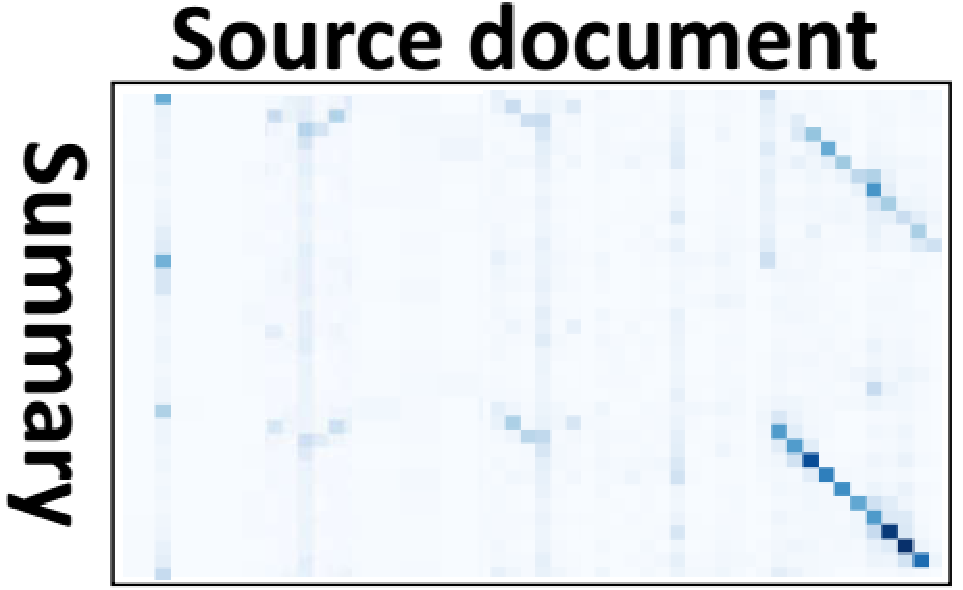
\includegraphics[width=0.16\linewidth]{mapITA}
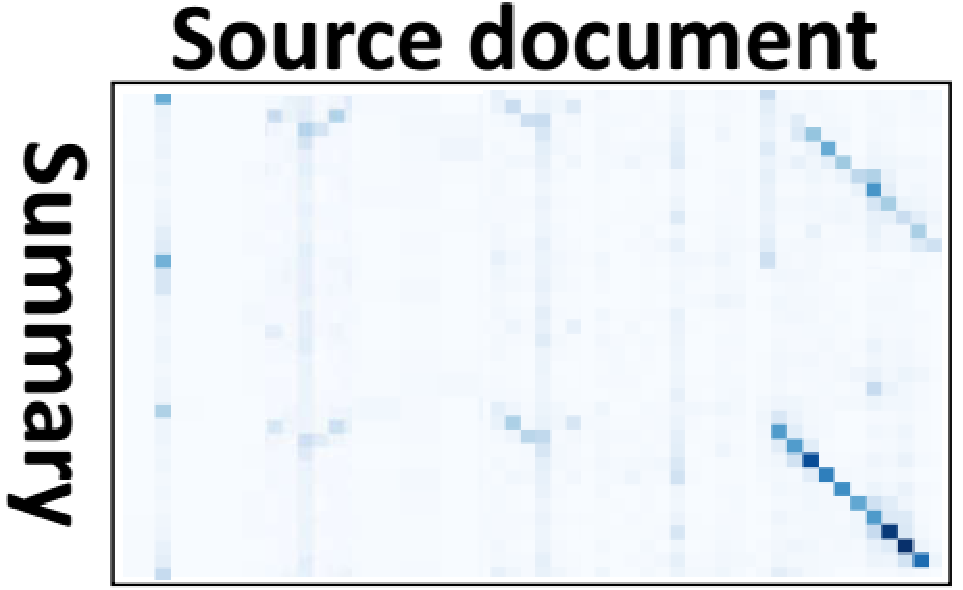
\includegraphics[width=0.26\columnwidth]{mapITA}
}
\quad
\subfigure[ITDA]{
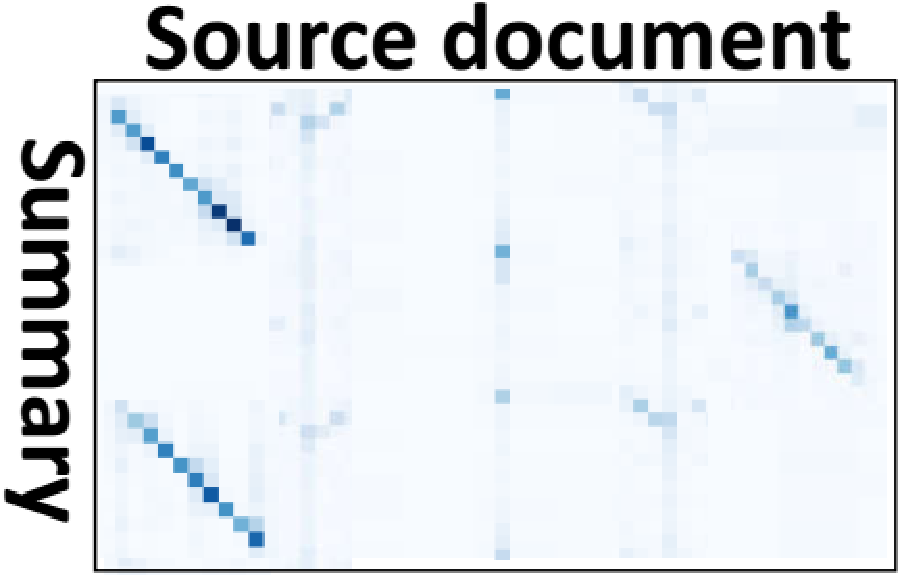
\includegraphics[width=0.26\linewidth]{mapITDA}
}
\quad
\subfigure[COV]{
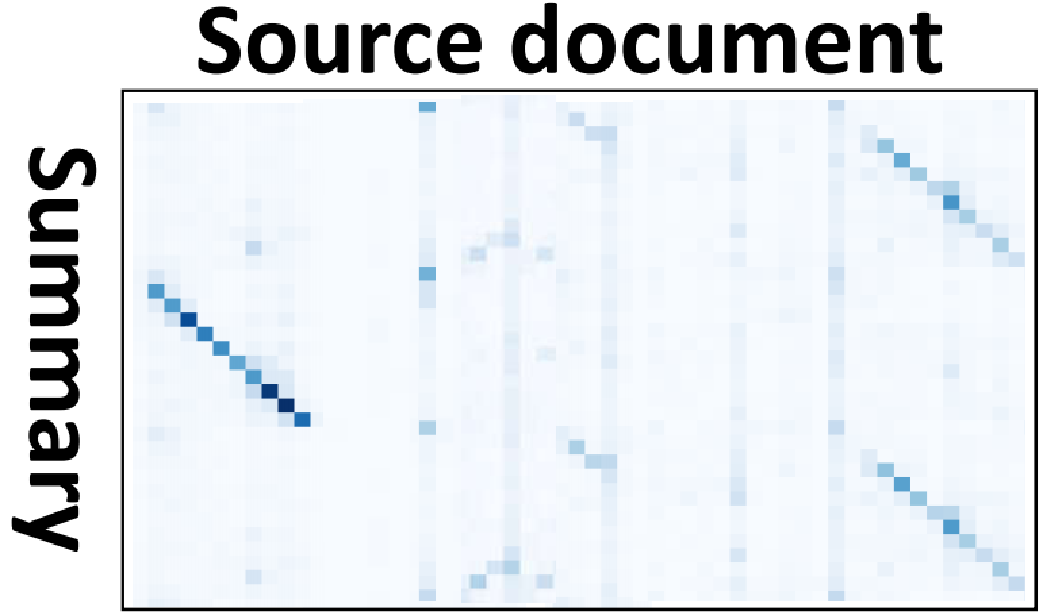
\includegraphics[width=0.26\linewidth]{mapCOV}
}
\quad
\subfigure[COVP]{
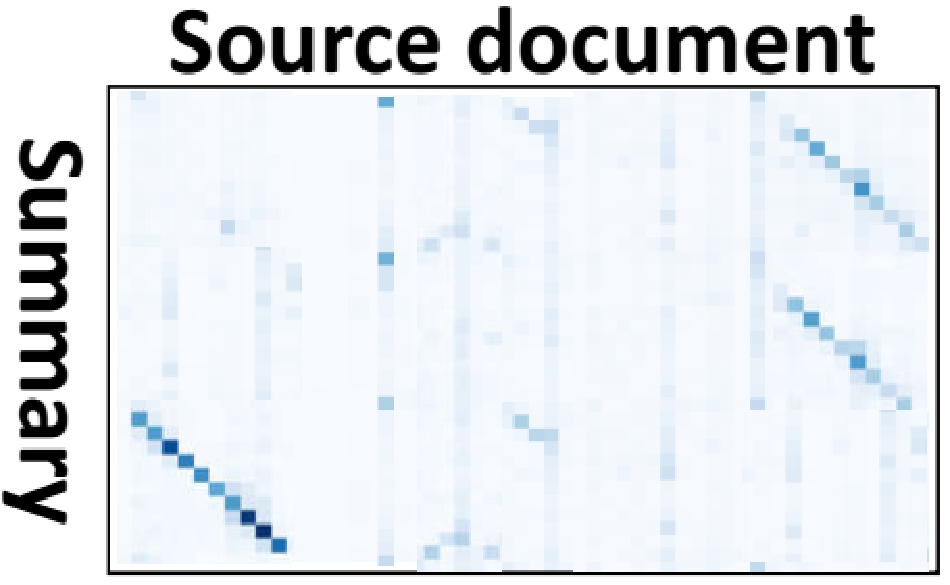
\includegraphics[width=0.26\linewidth]{mapCOVP}
}
\quad
\subfigure[SCL]{
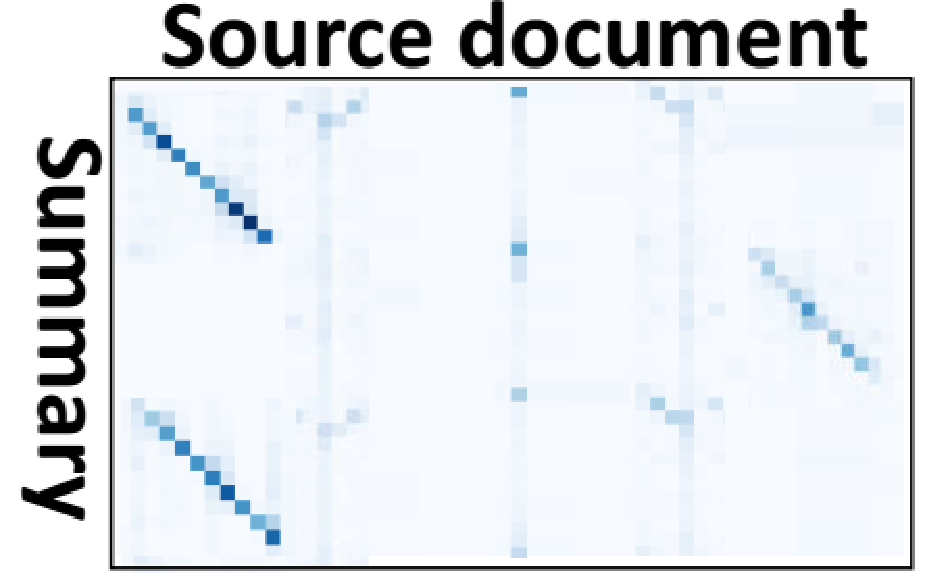
\includegraphics[width=0.26\linewidth]{mapSCL}
}
\quad
\subfigure[ATTF]{
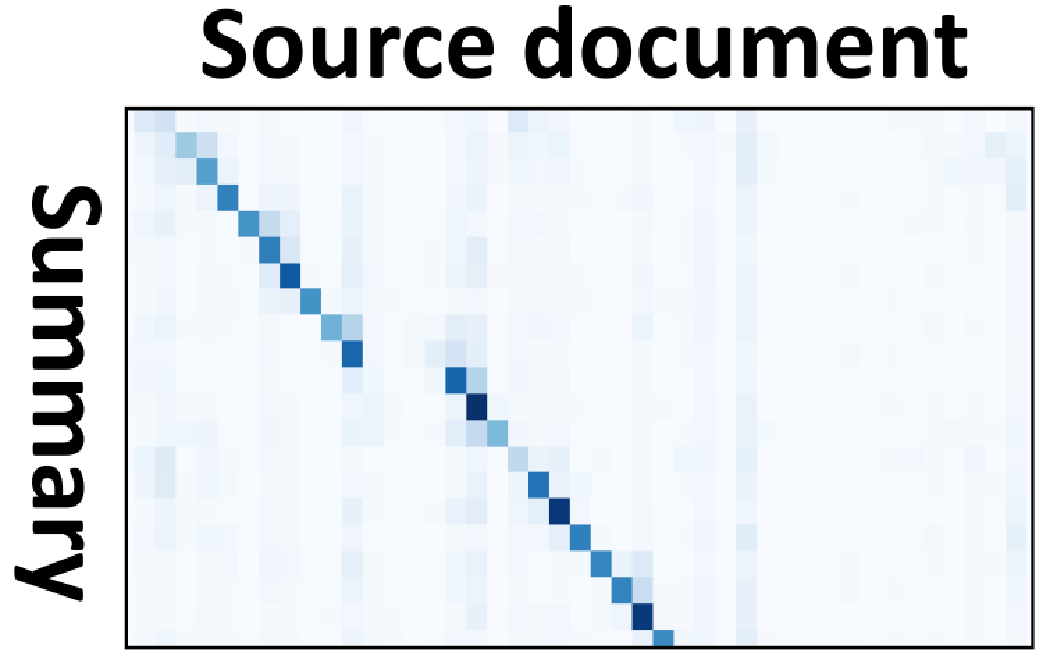
\includegraphics[width=0.26\linewidth]{map2}
}
%\caption{Attention distribution of examples in \tabref{tab:strong_methods}}
\caption{Attention distribution of summaries for the source in \tabref{tab:example}}
\label{fig:attn_maps}
\end{figure}

Compared with the Gold standard,
ATTF still generates some repetitive sentences,
due to similar sentences in source
such as \exref{ex:repeatsrc}.
%The result of summarizing that document using ATTF and its local attention map are
The summary generated by ATTF and its local attention are
shown in \tabref{tab:src_rep} and \figref{fig:attn_map3}.
Also, SBD further reduces the repetition when combined with ATTF. 
%which demonstrates its effectiveness.

\begin{table}[th!]
\begin{center}
\scriptsize
\begin{tabular}{|l|}%{|p{7cm}|rl|}
\hline \textbf{Reference:} oriol romeu is on a season-long loan at stuttgart from chelsea . \\
       the spanish midfielder predicts the scores in saturday 's matches . oriol goes \\
	   head-to-head with sportsmail 's martin keown .\\
\hline \textbf{ATTF:} chelsea beat manchester united on saturday . \textit{oriol romeu is currently} \\
       \textit{on a season-long loan at stuttgart . oriol romeu is currently on a season-long} \\
	   \textit{loan at bundesliga side stuttgart .}\\
\hline \textbf{SBD:} chelsea beat manchester united on saturday . chelsea face manchester \\
       united in the premier league . \\ 
\hline \textbf{ATTF+SBD:} chelsea face manchester united in the premier league on saturday . \\
       oriol romeu is currently on loan at stuttgart . \\
\hline
\end{tabular}
\end{center}
\caption{Summaries generated from \exref{ex:repeatsrc}.}
\label{tab:src_rep}
\end{table}

\cut{%%%%%%%%
\begin{figure}[th!]
\centering
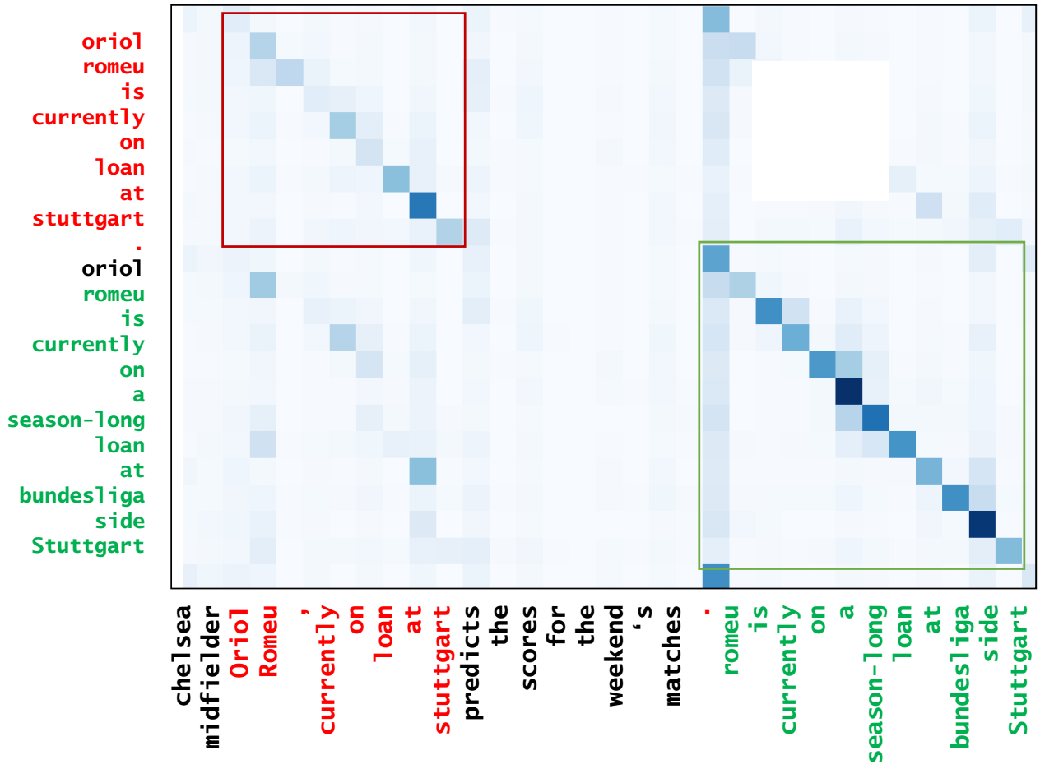
\includegraphics[width=0.84\columnwidth]{map3}
\caption{Attention distribution for ATTF in \tabref{tab:src_rep}}
\label{fig:attn_map3}
\end{figure}
}%%%%%%%%%%

As shown in \tabref{tab:eval_repe}, TRI has the lowest total repeatedness score.
It does not generate any repetitive N-grams (N$>$2) and sentences 
because TRI prevents the generation of the same trigrams during testing.
But as the Gold row shows, reference summaries do have some natural repetition.
%As reference summaries are human written, 
Therefore we evaluate the correlation of repeatedness distribution between
generated summaries and reference summaries (\tabref{tab:eval_repcor}).
Our proposed models \DIFdelbegin \DIFdel{achieve better results, among which ATTF+SBD performs best,
an indication }\DIFdelend \DIFaddbegin \DIFadd{perform best,
which indicates }\DIFaddend that ATTF and SBD are more capable of producing summaries with a natural level of repeatedness.
%It indicates that ATTF and SBD are more capable of producing summaries with a natural level of repeatedness.
%missing POIs and repetition in source documents.

\begin{table}[th!]
        \centering
        \small
        \begin{tabular}{|l|c|c|c|}
                \hline
                     & pearson  & spearman & kendall's tau \\
                \hline
                \DIFaddbeginFL \DIFaddFL{ATTF }& \bf \DIFaddFL{1.0 }& \bf \DIFaddFL{1.0 }& \bf \DIFaddFL{1.0 }\\
                \DIFaddendFL TRI* & 1.0 & \DIFdelbeginFL \DIFdelFL{0.894 }\DIFdelendFL \DIFaddbeginFL \DIFaddFL{0.89 }\DIFaddendFL & \DIFdelbeginFL \DIFdelFL{0.837  }\DIFdelendFL \DIFaddbeginFL \DIFaddFL{0.84  }\DIFaddendFL \\
                SBD* & \DIFaddbeginFL \bf \DIFaddendFL 1.0 & \DIFaddbeginFL \bf \DIFaddendFL 1.0 & \DIFaddbeginFL \bf \DIFaddendFL 1.0 \\
                %DIF < ATTF & 0.998 & 0.943 & 0.867 \\
                ATTF+TRI* & 1.0 & \DIFdelbeginFL \DIFdelFL{0.894 }\DIFdelendFL \DIFaddbeginFL \DIFaddFL{0.89 }\DIFaddendFL & \DIFdelbeginFL \DIFdelFL{0.837 }\DIFdelendFL \DIFaddbeginFL \DIFaddFL{0.84 }\DIFaddendFL \\
                ATTF+SBD* & \bf 1.0 & \bf 1.0 & \bf 1.0 \\
                \hline
        \end{tabular}
    \caption{Repeatedness correlation between generated summaries and Gold summaries.}
        \label{tab:eval_repcor}
\end{table}

\begin{figure}[th!]
\centering
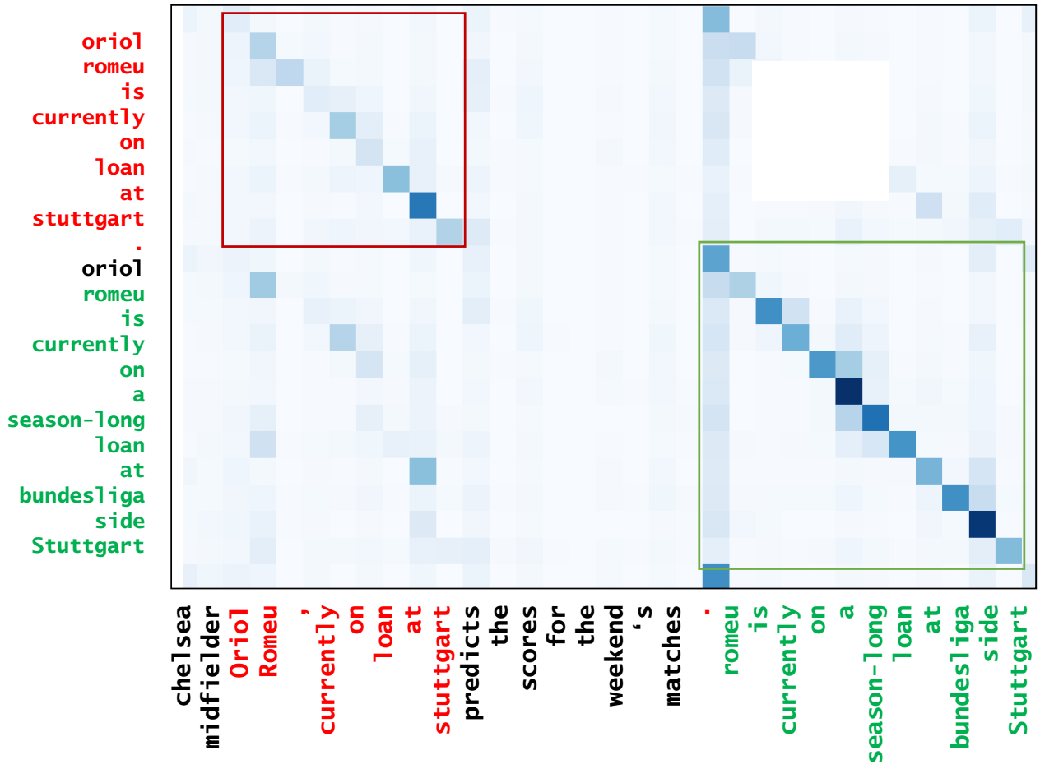
\includegraphics[width=0.84\columnwidth]{map3}
\caption{Attention distribution for ATTF in \tabref{tab:src_rep}}
\label{fig:attn_map3}
\end{figure}

\textbf{Readability.}
As shown in \tabref{tab:eval_repe}, 
the models with ATTF achieve the
%ATTF achieves the
highest readability score among all baselines, 
which means ATTF is more readable.
%without any operations during test.
TRI achieves the best score on repeatedness, 
% which represents the repetition over N-gram and sentences,
but lower readability score than other models.
Also, the readability of ATTF drops after adding TRI.
%All of our models score higher than $0.80$. 
SBD enhances performance of CNN and ATTF by reducing the repetitive unreadable sentences. 
ATTF+SBD scores highest on readability.
\DIFdelbegin %DIFDELCMD < \cut{%%%%%%%%%
%DIFDELCMD < \begin{table}[th!]
%DIFDELCMD < 	\centering
%DIFDELCMD < 	\small
%DIFDELCMD < 	\begin{tabular}{|l|c|c|c|}
%DIFDELCMD < 		\hline
%DIFDELCMD < 		     & pearson  & spearman & kendall's tau \\
%DIFDELCMD < 		\hline
%DIFDELCMD < 		TRI* & 1.0 & 0.894 & 0.837  \\
%DIFDELCMD < 		SBD* & 1.0 & 1.0 & 1.0 \\
%DIFDELCMD < 		%ATTF & 0.998 & 0.943 & 0.867 \\
%DIFDELCMD < 		ATTF+TRI* & 1.0 & 0.894 & 0.837 \\
%DIFDELCMD < 		ATTF+SBD* & \bf 1.0 & \bf 1.0 & \bf 1.0 \\
%DIFDELCMD < 		\hline
%DIFDELCMD < 	\end{tabular}
%DIFDELCMD <     \caption{Repeatedness correlation between generated summaries and Gold summaries.}
%DIFDELCMD < 	\label{tab:eval_repcor}
%DIFDELCMD < \end{table}
%DIFDELCMD < }%%%
\DIFdelend \DIFaddbegin \cut{%%%%%%%%%
\begin{table}[th!]
	\centering
	\small
	\begin{tabular}{|l|c|c|c|}
		\hline
		     & pearson  & spearman & kendall's tau \\
		\hline
		TRI* & 1.0 & 0.894 & 0.837  \\
		SBD* & 1.0 & 1.0 & 1.0 \\
		ATTF+TRI* & 1.0 & 0.894 & 0.837 \\
		ATTF+SBD* & \bf 1.0 & \bf 1.0 & \bf 1.0 \\
		\hline
	\end{tabular}
    \caption{Repeatedness correlation between generated summaries and Gold summaries.}
	\label{tab:eval_repcor}
\end{table}
}\DIFaddend %%%


\textbf{Speed.} 
As shown in \tabref{tab:eval_main} and \tabref{tab:eval_speed}, 
SBD is the best sentence-level backtracking decoder.

\begin{table}[th!]
\centering
\small
\begin{tabular}{|l|c|c|c|}
\hline
Model & Time (s) & summaries/s & tokens/s \\
\hline
RNN  &  21600 & 0.48 & 29.60 \\
FastRNN &  3600 & 2.92 & 219.60 \\
\hline
CNN &  346.1 & 30.36 & 1343.46 \\
SBD-b1 &  412.8 & 25.46 & 1126.38 \\
SBD-b2 &  843.5 & 12.16 & 551.24 \\
SBD &  912.8 & 11.51 & 493.68 \\
ATTF & 1332 & 7.89 &  349.00 \\
ATTF+SBD & 1832.3 & 5.74 &  253.77 \\
\hline
\end{tabular}
\caption{Testing time and speed of generation.}
\label{tab:eval_speed}
\end{table}


Compared with SBD-b1 and SBD-b2,
SBD logs higher ROUGE score without losing much on speed. 
We compare the speed of our model to RNN~\cite{SeeLM17} and FastRNN~\cite{P18-1063}
which used K40. 
We perform experiments on GTX-1080ti and scale the speed 
reported for the RNN methods,
since GTX-1080ti is twice as fast as K40~\cite{gehring2017convs2s}.
Our model can 
generate summaries much faster than previous RNN seq2seq models.
%FastRNN is also fast because 

\DIFdelbegin %DIFDELCMD < \cut{%%%%%%%%%%%
%DIFDELCMD < \begin{table}[th!]
%DIFDELCMD < \centering
%DIFDELCMD < \small
%DIFDELCMD < \begin{tabular}{|l|c|c|c|}
%DIFDELCMD < \hline
%DIFDELCMD < Model & Time (s) & summaries/s & tokens/s \\
%DIFDELCMD < \hline
%DIFDELCMD < RNN  &  21600 & 0.48 & 29.60 \\
%DIFDELCMD < FastRNN &  3600 & 2.92 & 219.60 \\
%DIFDELCMD < \hline
%DIFDELCMD < CNN &  346.1 & 30.36 & 1343.46 \\
%DIFDELCMD < SBD-b1 &  412.8 & 25.46 & 1126.38 \\
%DIFDELCMD < SBD-b2 &  843.5 & 12.16 & 551.24 \\
%DIFDELCMD < SBD &  912.8 & 11.51 & 493.68 \\
%DIFDELCMD < ATTF & 1332 & 7.89 &  349.00 \\
%DIFDELCMD < ATTF+SBD & 1832.3 & 5.74 &  253.77 \\
%DIFDELCMD < \hline
%DIFDELCMD < \end{tabular}
%DIFDELCMD < \caption{Testing time and speed of generation.}
%DIFDELCMD < \label{tab:eval_speed}
%DIFDELCMD < \end{table}
%DIFDELCMD < }%%%
%DIF < %%%%%%%%%%%%%
%DIFDELCMD < 

%DIFDELCMD < %%%
\DIFdelend %\subsection{Significance Test on ROUGE scores}
\DIFaddbegin \begin{table}[th!]
\begin{center}
\small
		\begin{tabular}{|l|c|c|c|}
		\hline
		\DIFaddFL{Model }&   \DIFaddFL{R-1 }& \DIFaddFL{R-2 }& \DIFaddFL{R-L }\\
		\hline
		\DIFaddFL{CNN }&  \DIFaddFL{2.32e-35 }& \DIFaddFL{6.34e-48 }& \DIFaddFL{3.68e-10 }\\
		\DIFaddFL{ITA }&  \DIFaddFL{6.14e-34 }& \DIFaddFL{2.12e-48 }& \DIFaddFL{5.67e-12 }\\
		\DIFaddFL{ITDA }& \DIFaddFL{2.76e-32 }& \DIFaddFL{4.52e-44 }& \DIFaddFL{3.94e-12 }\\
		\DIFaddFL{COV	}& \DIFaddFL{4.14e-30 }& \DIFaddFL{4.61e-50 }& \DIFaddFL{7.12e-12 }\\
		\DIFaddFL{COVP }& \DIFaddFL{2.51e-32 }& \DIFaddFL{3.17e-41 }& \DIFaddFL{2.15e-10 }\\
		\DIFaddFL{SCL	}& \DIFaddFL{3.11e-32 }& \DIFaddFL{3.29e-44 }& \DIFaddFL{3.43e-15 }\\
		\DIFaddFL{TRI }& \DIFaddFL{5.25e-30 }& \DIFaddFL{1.33e-43 }& \DIFaddFL{3.67e-12 }\\
		\hline
		\end{tabular}
\caption{\DIFaddFL{p-value of significance test between 
our best proposed model (ATTF+SBD) and baselines on ROUGE scores}}
\label{tab:ttest}
\end{center}
\end{table}
\DIFaddend 

\textbf{Significance Test.} We use significance test to prove that the ROUGE scores in \tabref{tab:eval_main} is reliable.
We take \DIFdelbegin \DIFdel{Kruskal-Wallis test }\DIFdelend \DIFaddbegin \DIFadd{t-test 
}\DIFaddend \cite{loukina2014automatic,albert2017exploring}
as our significance test to
measure that the ROUGE scores \DIFaddbegin \DIFadd{between our proposed approach (ATTF+SBD) and each baseline }\DIFaddend are significant or not. 
As shown in \DIFdelbegin %DIFDELCMD < \tabref{tab:pvalue}%%%
\DIFdelend \DIFaddbegin \tabref{tab:ttest}\DIFaddend ,
all p-values are less than 0.05. 
The smaller p-value, the higher significant.
Thus, the difference of the similarity results is significant. 
				%DIF < \YZ{table for significance test}


\DIFdelbegin \DIFdel{The }\DIFdelend \DIFaddbegin \DIFadd{Overall, the }\DIFaddend summaries generated by sequence-to-sequence models with attention mechanism always contain repetition.  
Through our observations, there are two reasons for repetition in abstractive summarization.
One is that the traditional attention mechanisms attend to the same location in source document at decoding.
The other is that the attention mechanism attend to the repetitive sentences in different locations in source document. 
As shown in \figref{fig:attn_maps} and \tabref{tab:src_rep},
our proposed ATTF and SBD effectively solve above two problems.  
The higher ROUGE scores (\tabref{tab:eval_main}) of our model means that
the summaries generated by our model are more similar to their corresponding reference summaries.
The natural-level repeatedness and higher readability score (\tabref{tab:eval_repe}) of our model means 
that our model can produce \DIFdelbegin \DIFdel{higher quality summaries}\DIFdelend \DIFaddbegin \DIFadd{summaries with higher quality}\DIFaddend .
Thus, our model can improve the reading speed and accuarcy of reading comprehension.



\section{Conclusion}
\label{sec:conclude}
%DIF < We presented a distributed attention mechanism to modify existing CNN seq2seq model 
%DIF < and were able to train a model that produces 
%DIF < summaries without repetition that are fluent and coherent. 
We analyze two possible reasons behind the repetition problem in abstractive
summarization: (1) attending to the same location in source,
and (2) attending to similar but different sentences in source. 
In response, we present a section-aware attention mechanism (ATTF)
as well as a sentence-level backtracking decoder (SBD). 
\DIFdelbegin \DIFdel{Our }\DIFdelend %DIF > Compared ,we presented a distributed attention mechanism to modify existing CNN seq2seq model 
%DIF > and were able to train a model that produces 
%DIF > The proposed models are able to train a model that produces 
%DIF > summaries without repetition that are fluent and coherent. 
\DIFaddbegin \DIFadd{The proposed }\DIFaddend model is able 
to produce \DIFaddbegin \DIFadd{more }\DIFaddend fluent and coherent summaries with minimal repetitions.
\DIFdelbegin \DIFdel{Besides, }\DIFdelend %DIF > Besides, 
\DIFaddbegin \DIFadd{It means that }\DIFaddend the summaries generated by our model are more accurate and 
readable\DIFaddbegin \DIFadd{. This can help user quickly get the main information from large of textual data,
saving the reading time and improving reading efficiency.
As some other natural language generation (NLG) tasks based on seq2seq model with attention mechanism
are orthogonal to our proposed methods,
they can also be enhanced with redistributed attention and repetition reduction}\DIFaddend .
%We find that the basic CNN seq2seq model 
%still has some problems, such as generating repeated word sequence. 
%We also argue that ROUGE is not a perfect evaluation metric for the abstractive 
%summarization. Our future work will focus on these two aspects.



\section*{References}

\bibliography{mybibfile}
\end{document}
